\documentclass[12pt,a4paper]{article}

% created by zcs at 2013-11-11
% Use XeLaTeX to compile.

% Package
\usepackage{amssymb}
\usepackage{fontspec}
\usepackage{xkeyval}
\usepackage[SlantFont,BoldFont,CJKchecksingle,CJKnumber]{xeCJK}
\usepackage{graphicx}
\usepackage{geometry}
\usepackage{fancyhdr}
\usepackage{lastpage}
\usepackage{indentfirst}
\usepackage{setspace}
\usepackage{titlesec}
\usepackage[normalem]{ulem}
\usepackage[CJKbookmarks]{hyperref}
\usepackage{float}
%\usetikzlibrary{mindmap} % LATEX and plain TEX
\usepackage{abstract}
\usepackage{listings}
\usepackage{enumerate}

%listing 设置 
\lstset{
  %backgroundcolor=\color{gray!25},
  numbers=left, numberstyle=\tiny\color{gray},numberblanklines=false,
  frame=single,
  basicstyle=\ttfamily,
  breaklines=true,
  escapechar=`,
  columns=fullflexible
}

% Page
\geometry{hmargin=3.2cm,top=4cm,bottom=3.2cm,headsep=1.2cm,footskip=1.2cm}

% Head & Foot
\pagestyle{fancy}
\lhead{惠理和奇虎回测结果 }
\chead{张昌盛}
\rhead{\href{mailto:changsheng.zhang@nedugroup.com}{changsheng.zhang}}
\lfoot{}
\cfoot{\thepage/\pageref{LastPage}}
\rfoot{}

% Paragraph
\setlength{\parindent}{2.45em}
\onehalfspacing

% Font
\newcommand\fontnamesong{SimSun}
\newcommand\fontnamehei{SimHei}
\newcommand\fontnamekai{KaiTi}
\newcommand\fontnameyahei{微软雅黑}
\newcommand\fontnameli{LiSu}

\defaultfontfeatures{Mapping=tex-text}
\setCJKmainfont[BoldFont=\fontnamehei, ItalicFont=\fontnamekai]{\fontnamesong}
\setCJKmonofont{\fontnameyahei}
\setCJKsansfont[BoldFont=\fontnamehei]{\fontnameyahei}
\XeTeXlinebreaklocale "zh"
\XeTeXlinebreakskip = 0pt plus 1pt

% Define fontfamily
\setCJKfamilyfont{song}{SimSun}
\setCJKfamilyfont{hei}{SimHei}
\newcommand\hei[1]{{\CJKfamily{hei}#1}}
\setCJKfamilyfont{kai}{KaiTi}
\newcommand\kai[1]{{\CJKfamily{kai}#1}}
\setCJKfamilyfont{yahei}{Microsoft YaHei}
\setCJKfamilyfont{li}{LiSu}
\setCJKfamilyfont{arial}{Arial}
\setCJKfamilyfont{fs}{FangSong}
%\newcommand\fs[1]{{\CJKfamily{fs}#1}}

% ULine
\renewcommand{\ULthickness}{1.5pt}
\setlength{\ULdepth}{4pt}

% Section
\titleformat{\section}{\centering\Huge\bfseries}{}{1em}{}
\renewcommand{\contentsname}{目录}
\renewcommand{\figurename}{图}
\renewcommand\refname{参考资料}
\renewcommand{\tablename}{表}
%\renewcommand\bibname{文献}
\renewcommand{\abstractname}{摘要}

% Hyperlink
\hypersetup{CJKbookmarks,bookmarksnumbered,colorlinks=true, linkcolor=black,
            citecolor=black,urlcolor=black, plainpages=false, pdfstartview=FitH}

\newenvironment{chkeyword}{{\hei{\xiaosi{关键词:}}}}  %定义中文关键词

%Table
\usepackage{multirow}
\usepackage{array}
\usepackage{multicol}
\usepackage{colortbl}
\usepackage[usenames,dvipsnames]{xcolor}

% Title
\title{惠理和奇虎回测结果}
\author{张昌盛}
\date{\today}

%%%%%%%%%%%%%%%%%%%%%%%%%%%%%%%%%%%%%%%%%%%%%%%%%%%%%%%%%%%%%%

\begin{document}
 

% Title page
\begin{titlepage}

\vspace{6pt}
\begin{center}
{\huge \fontsize{24bp}{\baselineskip}\CJKfamily{hei} 惠理和奇虎回测结果 }
\end{center}

\hspace{270pt}
{\fontsize{16bp}{\baselineskip}\CJKfamily{fs} \href{mailto:changsheng.zhang@nedugroup.com}{changsheng.zhang@nedugroup.com}}

\normalsize

\tableofcontents

\end{titlepage}

\newpage

\section{回测策略}

\subsection{4天动量模型}
\begin{enumerate}
\item 如果当天收盘价比4天前的收盘价高,则做多。(如果已经有多仓了,则继续持有多仓)
\item 如果当天收盘价比4天前的收盘价低,则做空。(如果已经有空仓了,则继续持有空仓)

\end{enumerate}

\subsection{量价模型}

\begin{enumerate}
\item 在股价上涨且成交量放大时买入;在其他条件时卖出(反手做空)
\item 为了减小波动,实际处理的数据对象是:M日平均收盘价和M日平均成交量(M可调,取1、2、5、7和10)
\item 股价上涨和成交放量的定义:最近N天的M日平均收盘价或者M日平均成交量的线性回归的斜率为正,则定义为上涨(放量),反之为下跌(缩量)。

\end{enumerate}

\section{回测结果}

\subsection{4天动量模型}

\begin{enumerate}
\item 回测时间是从2015年8月1日开始,日线;
\item 手续费0.1\%,买入卖出分别征收,策略为long/short和long/hold;
\end{enumerate}

\subsubsection{惠理}

\begin{figure}[H]
	\centering
	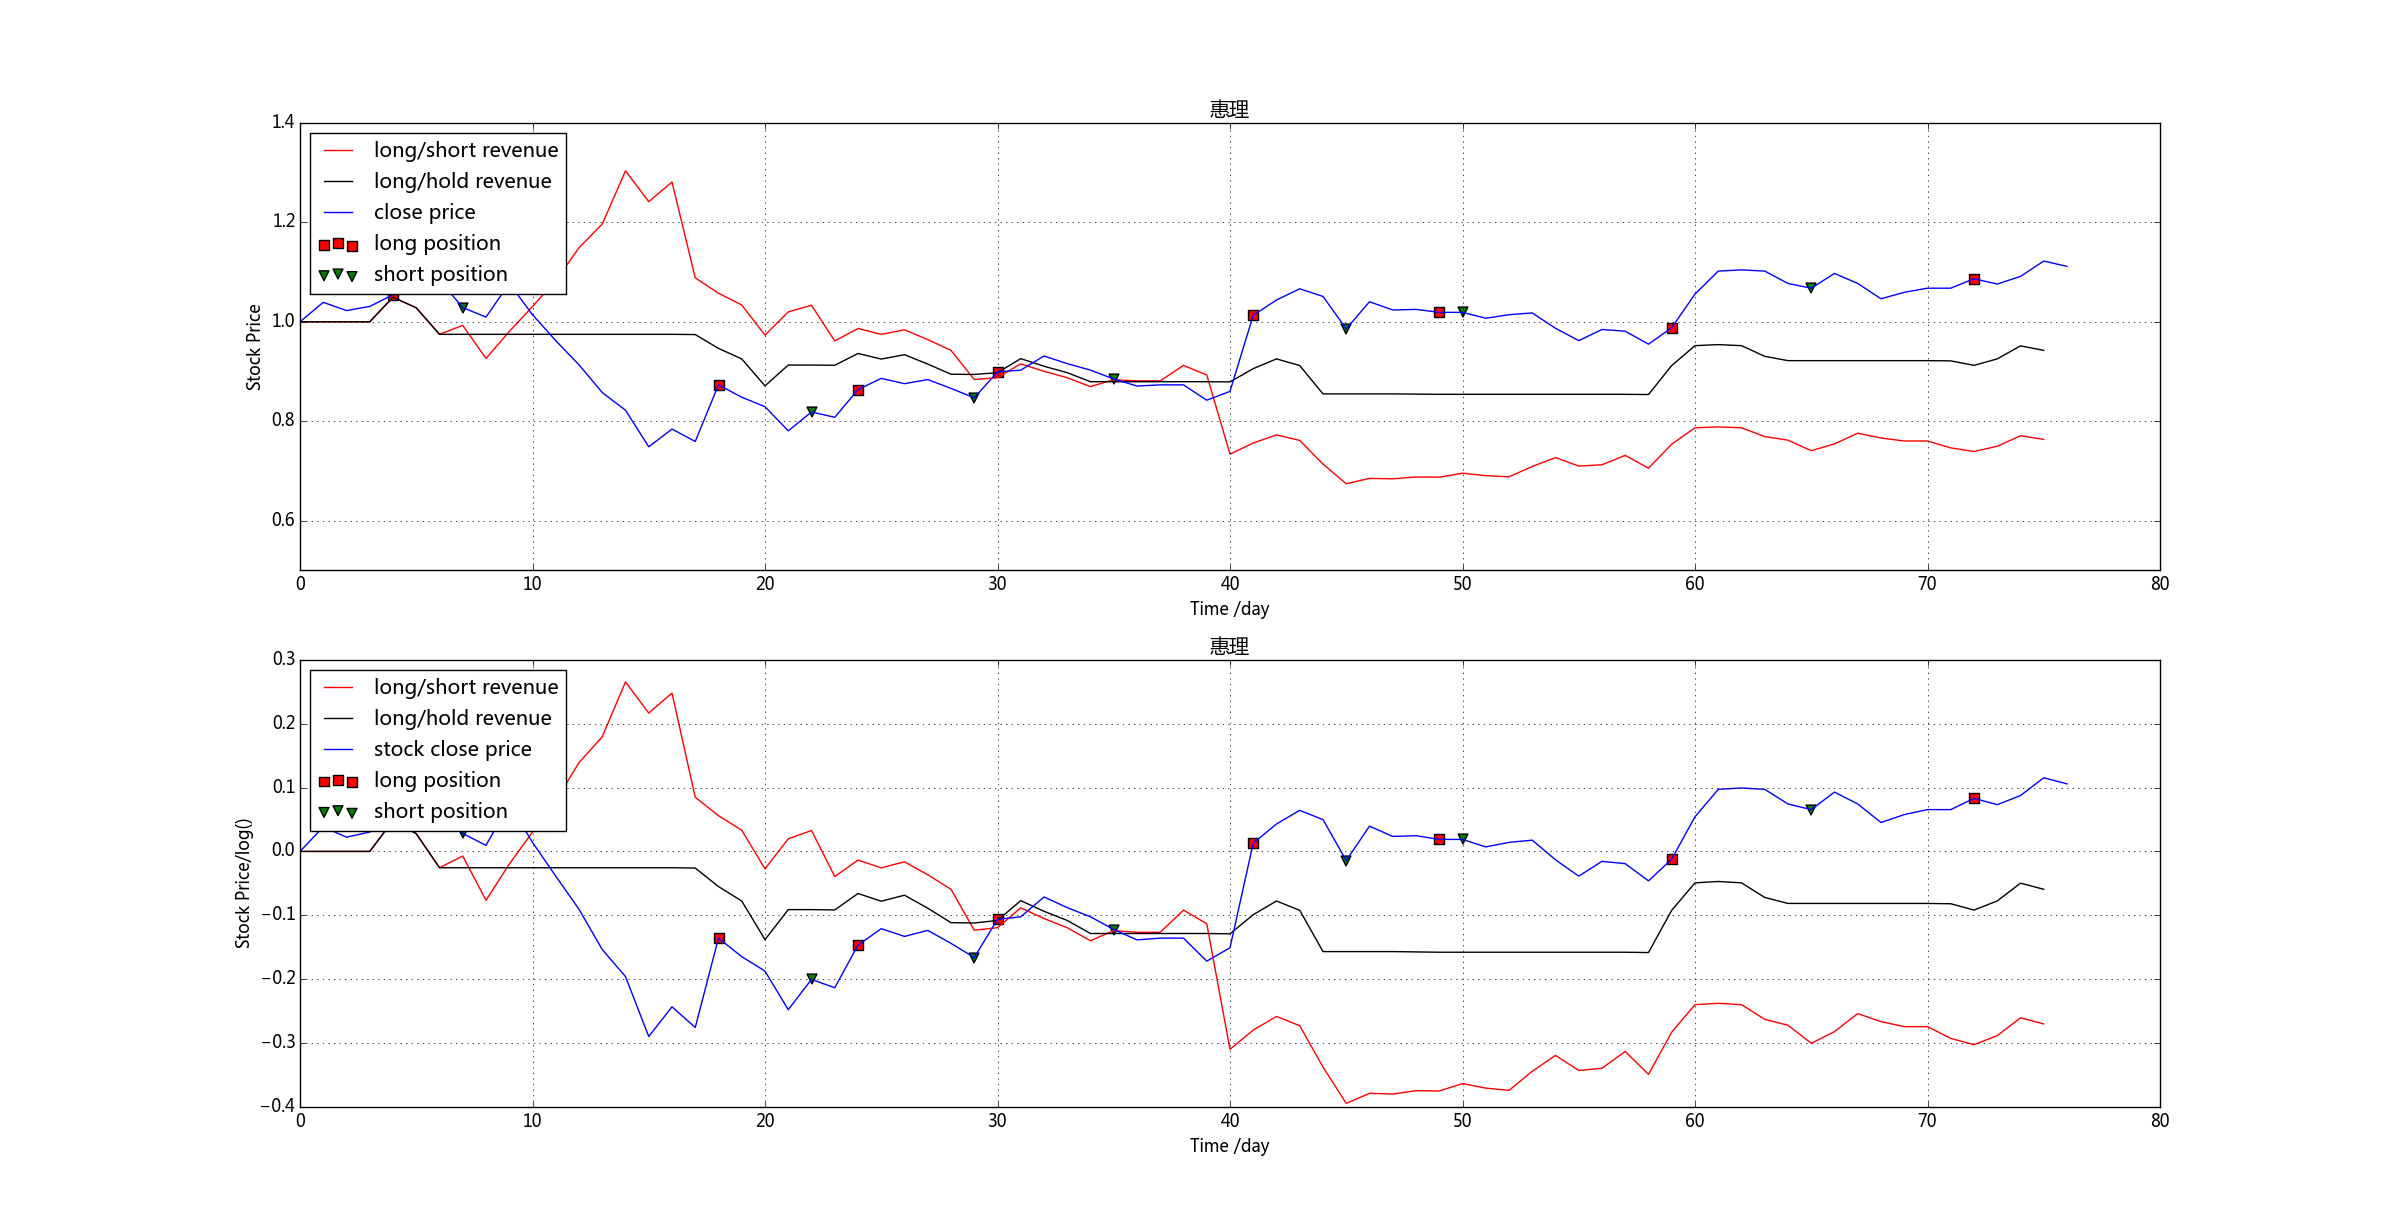
\includegraphics[width=1.0\textwidth]{img/0806.hk.png}
	\caption{惠理回测结果}
\end{figure}


\subsubsection{奇虎}

\begin{figure}[H]
	\centering
	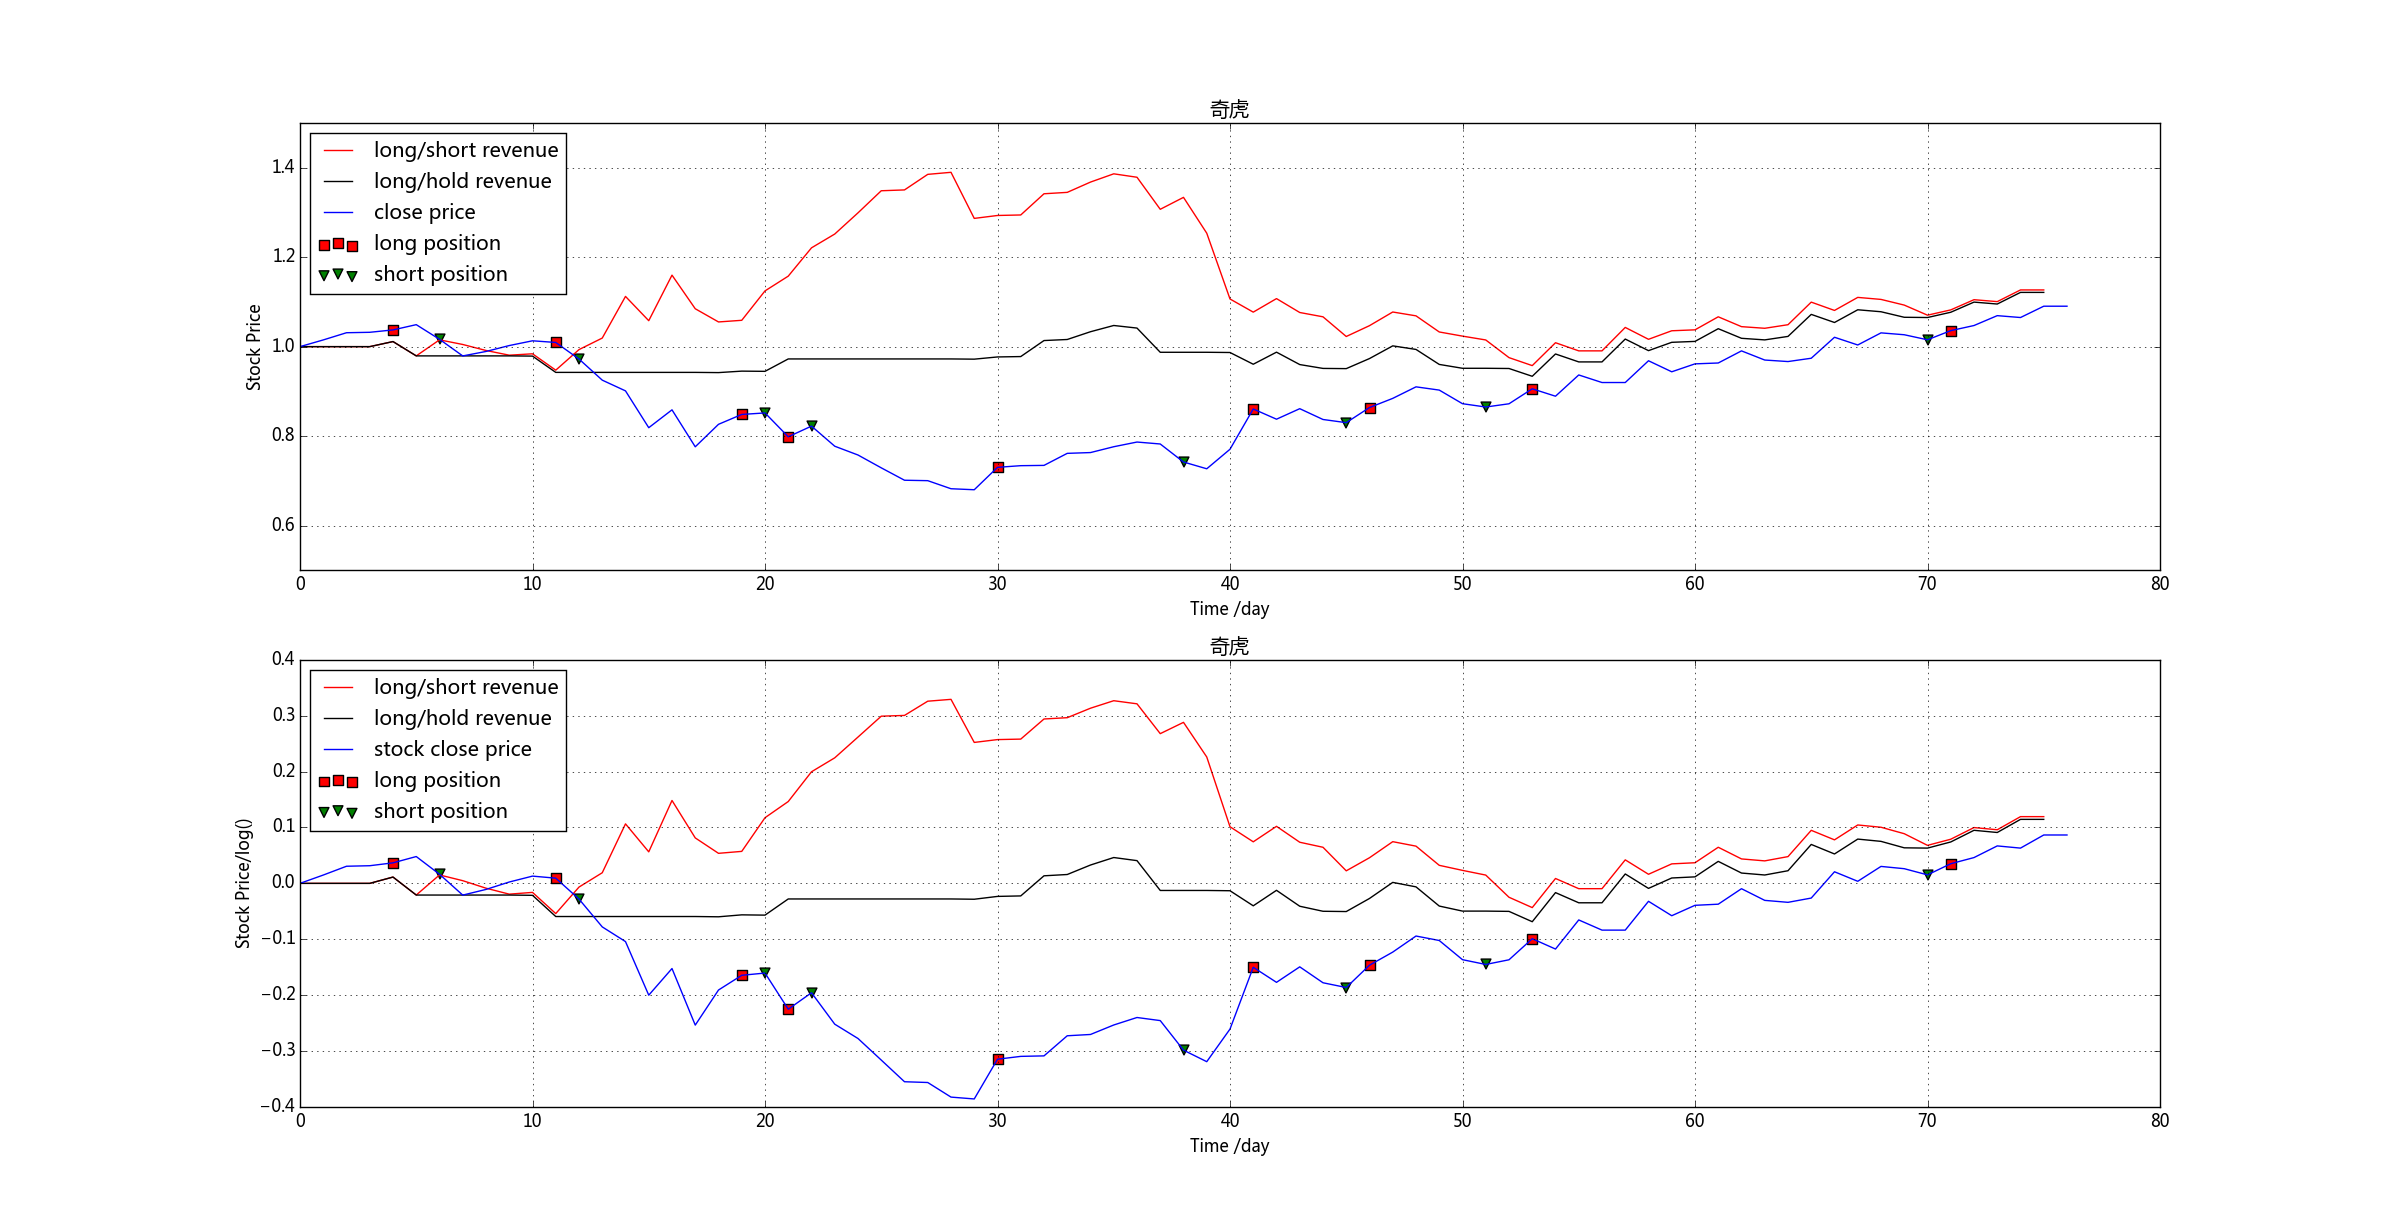
\includegraphics[width=1.0\textwidth]{img/qihu.n.png}
	\caption{奇虎回测结果}
\end{figure}

\subsection{量价模型}

\begin{enumerate}
\item 回测时间是从2015年8月1日开始,日线;
\item 手续费0.1\%,买入卖出分别征收,策略为long/short和long/hold;
\item 对股价和成交量做1(即不处理)、2和5日平均处理,线性回归处理的区间为2、5、7和10日。
\end{enumerate}


\subsubsection{价格和成交量1日MA(即不处理)}

\begin{enumerate}[1.]
\item 惠理 long/short


\begin{figure}[H]
	\centering
	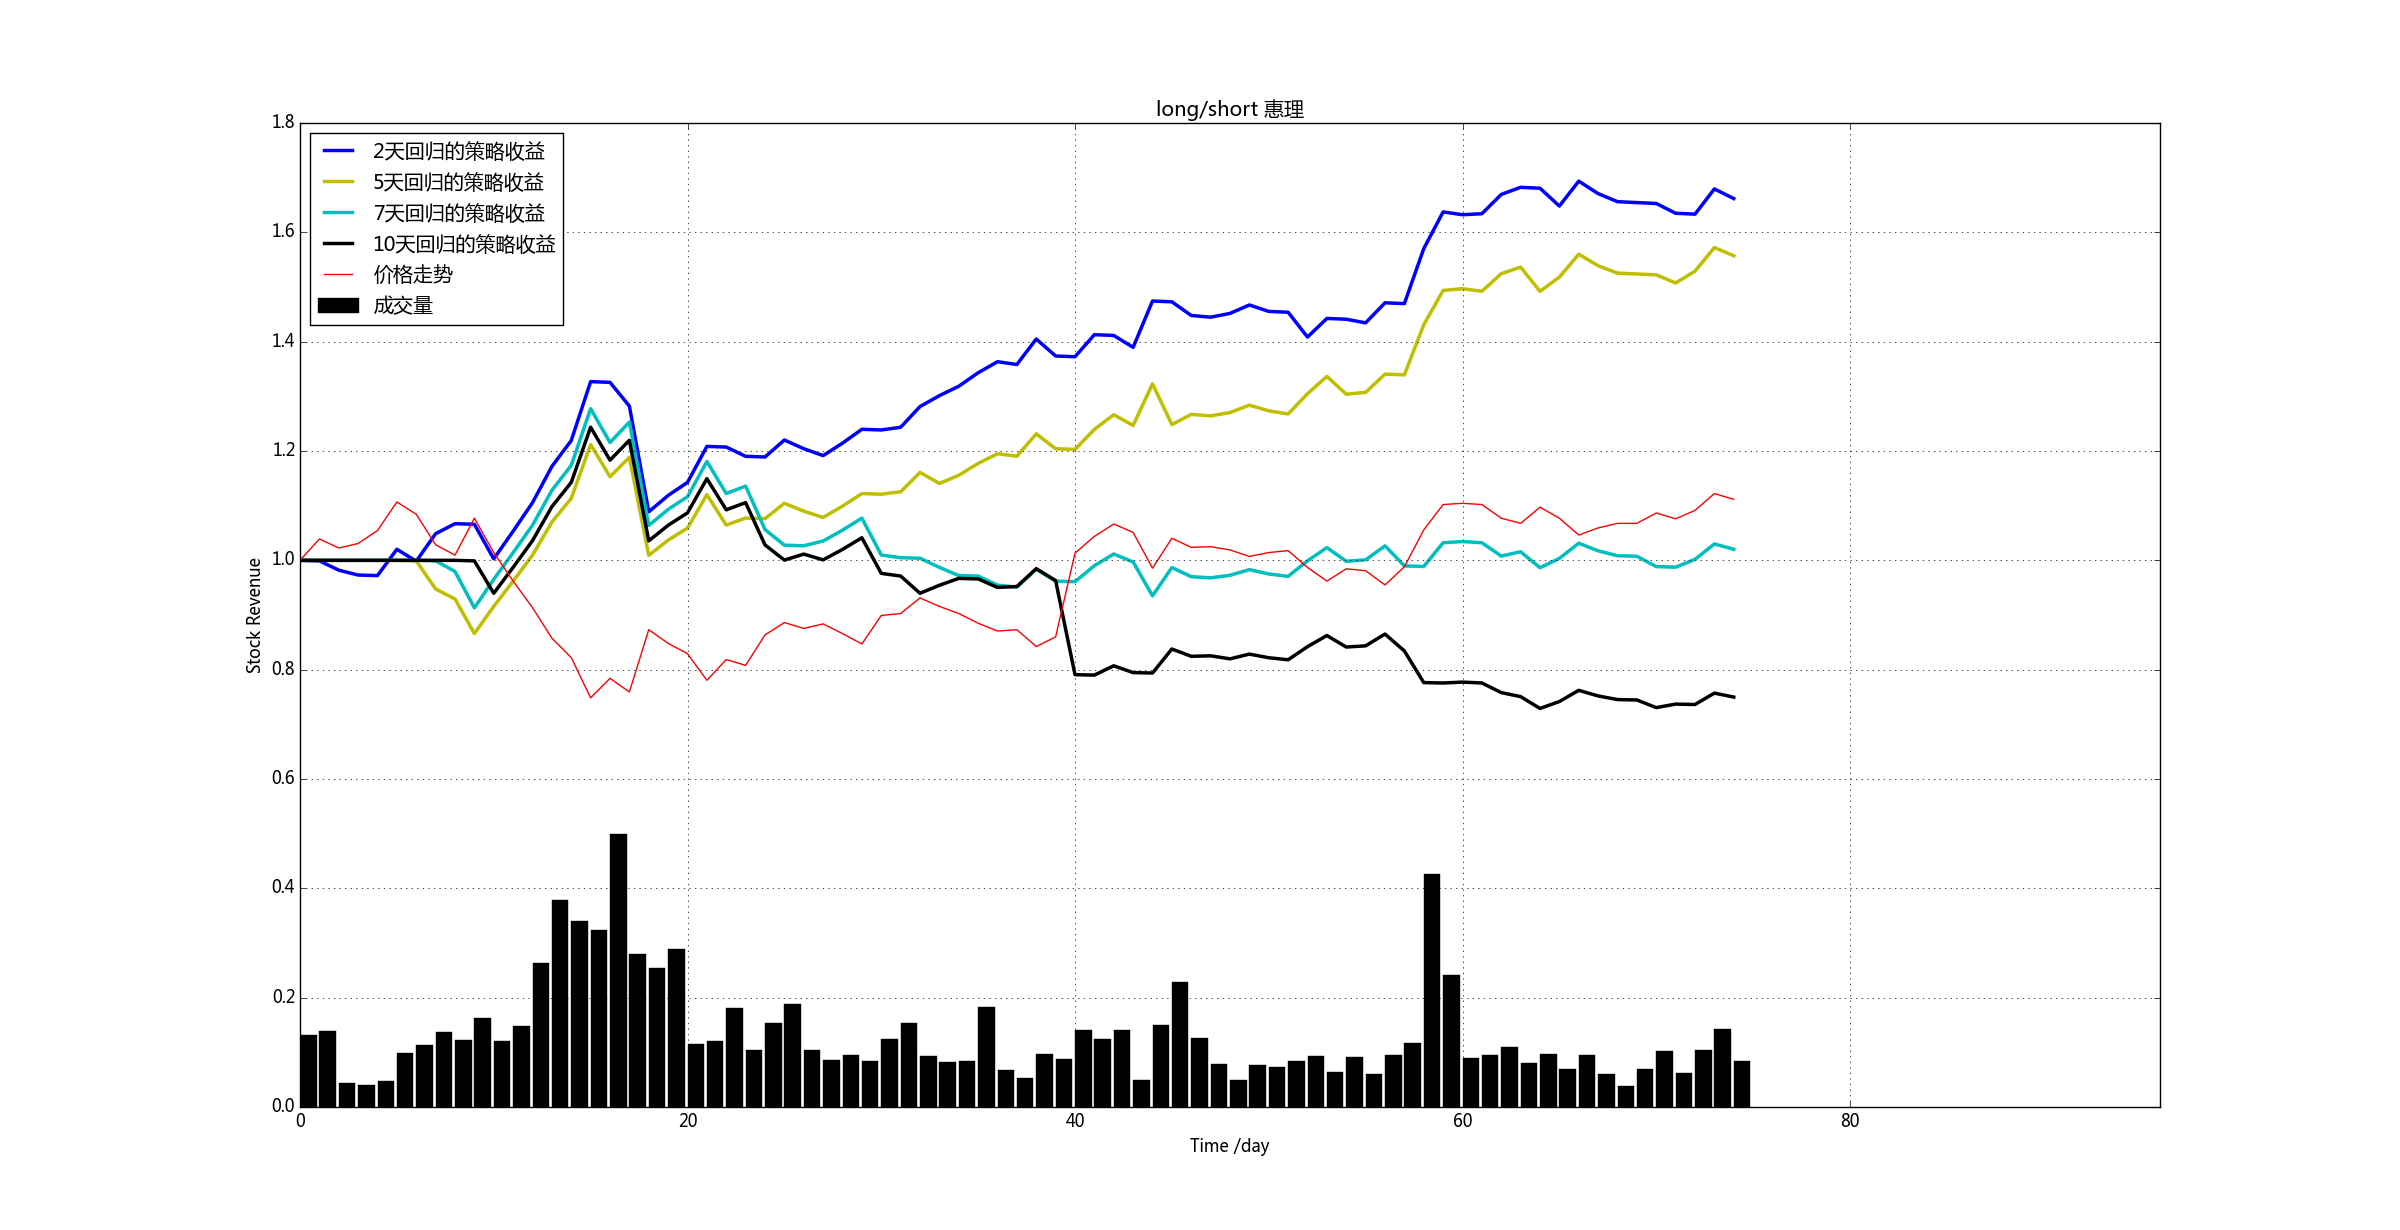
\includegraphics[width=1.0\textwidth]{img_r_1/short/hl.png}
	\caption{惠理 long/short}
\end{figure}

\item 惠理 long/hold

\begin{figure}[H]
	\centering
	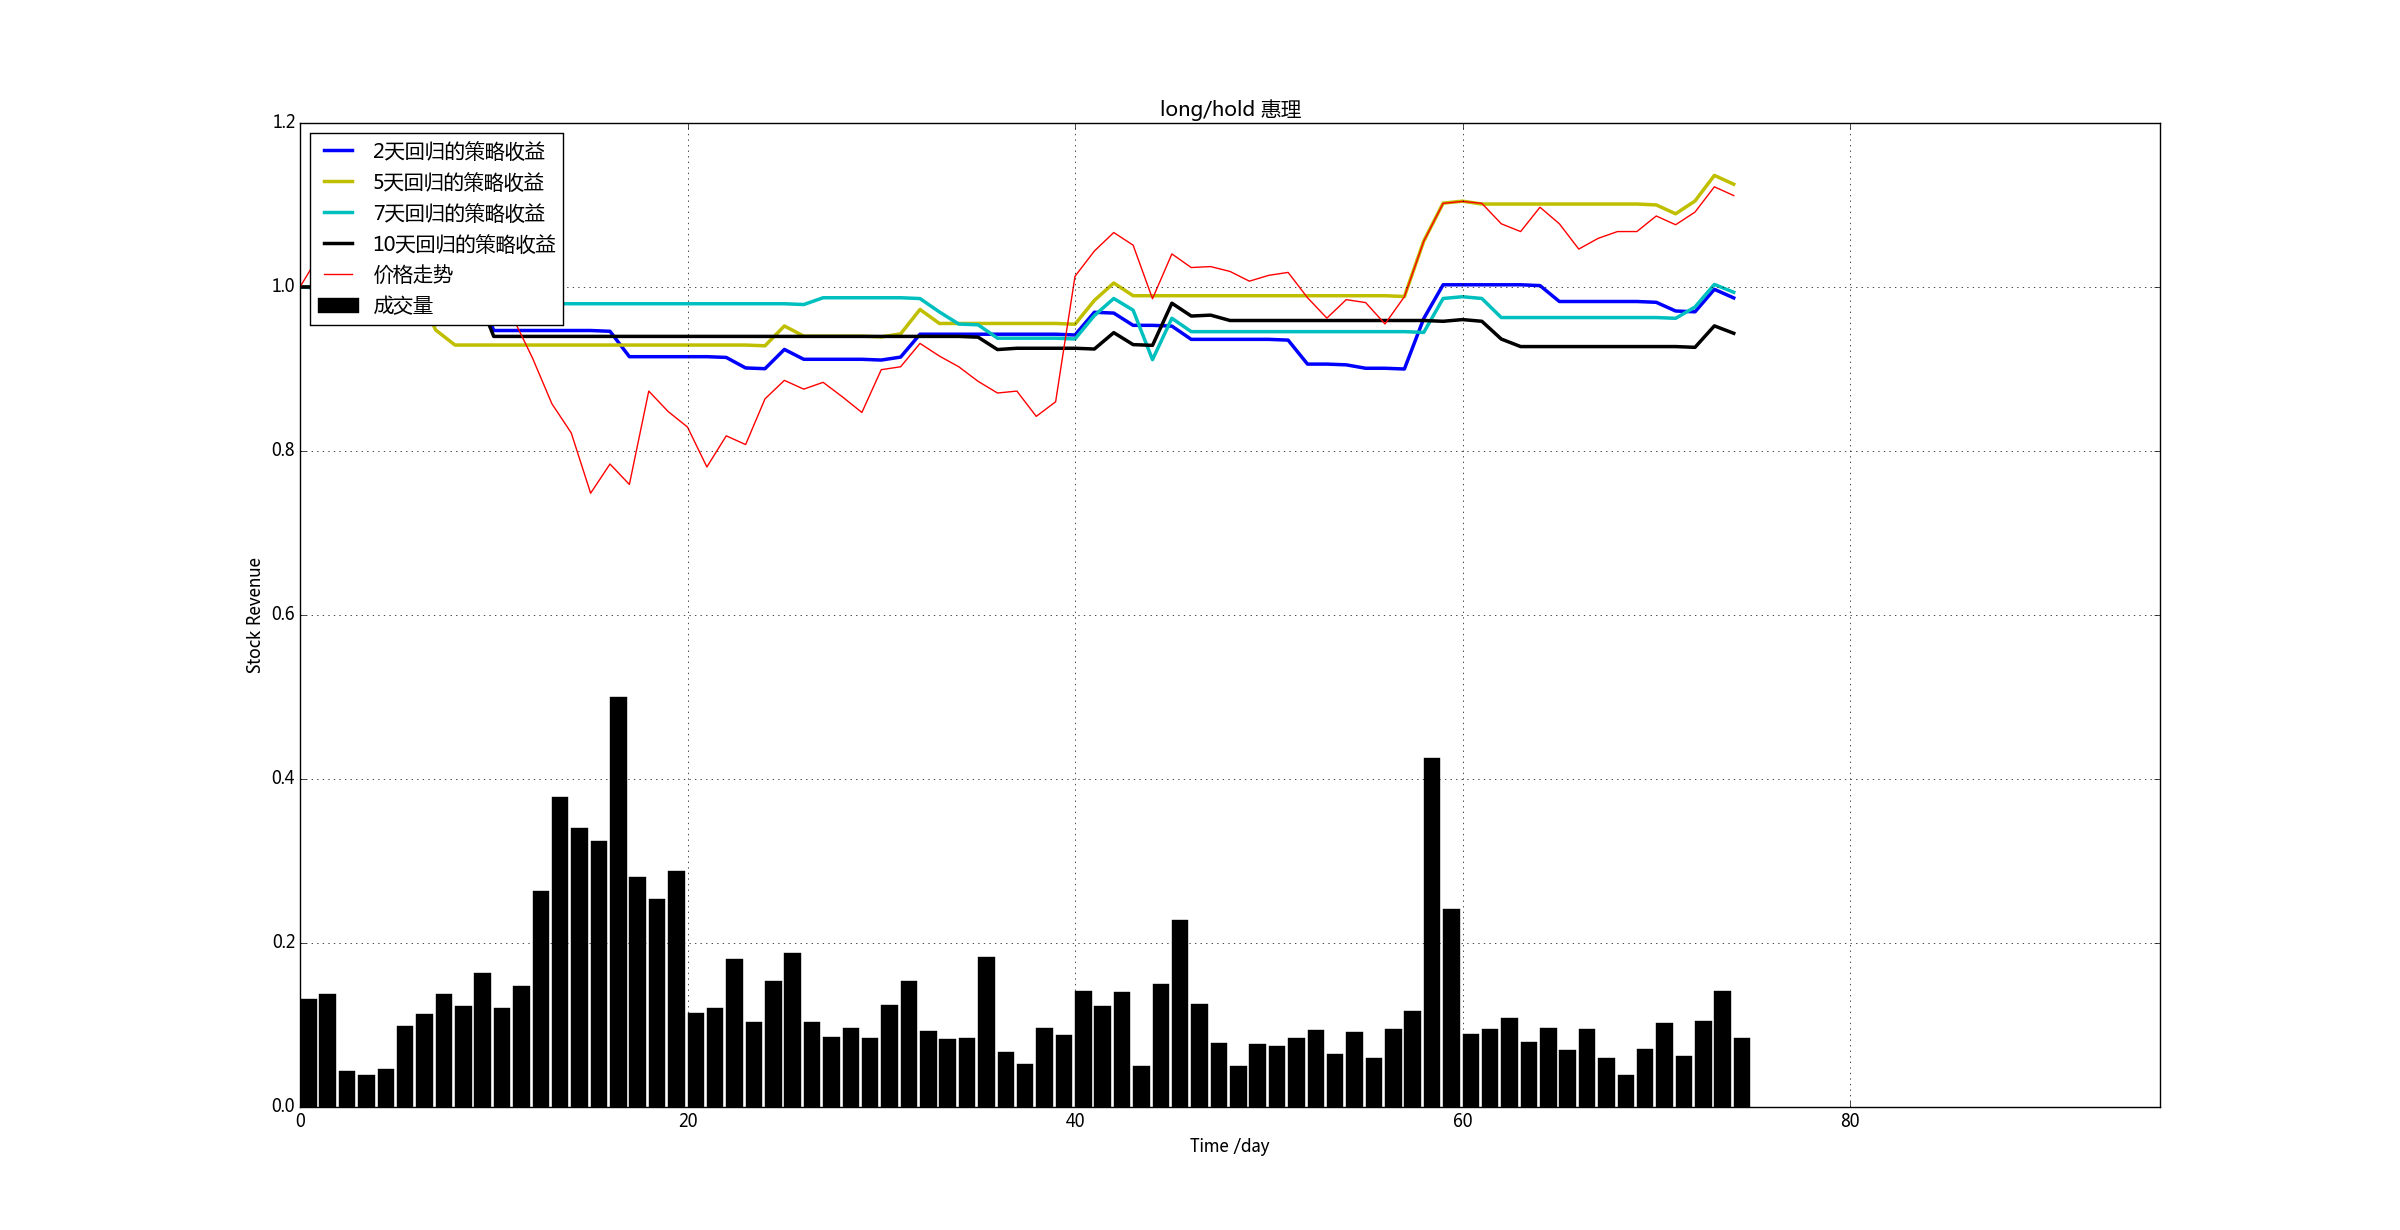
\includegraphics[width=1.0\textwidth]{img_r_1/hold/hl.png}
	\caption{惠理 long/hold}
\end{figure}

\item 奇虎 long/short


\begin{figure}[H]
	\centering
	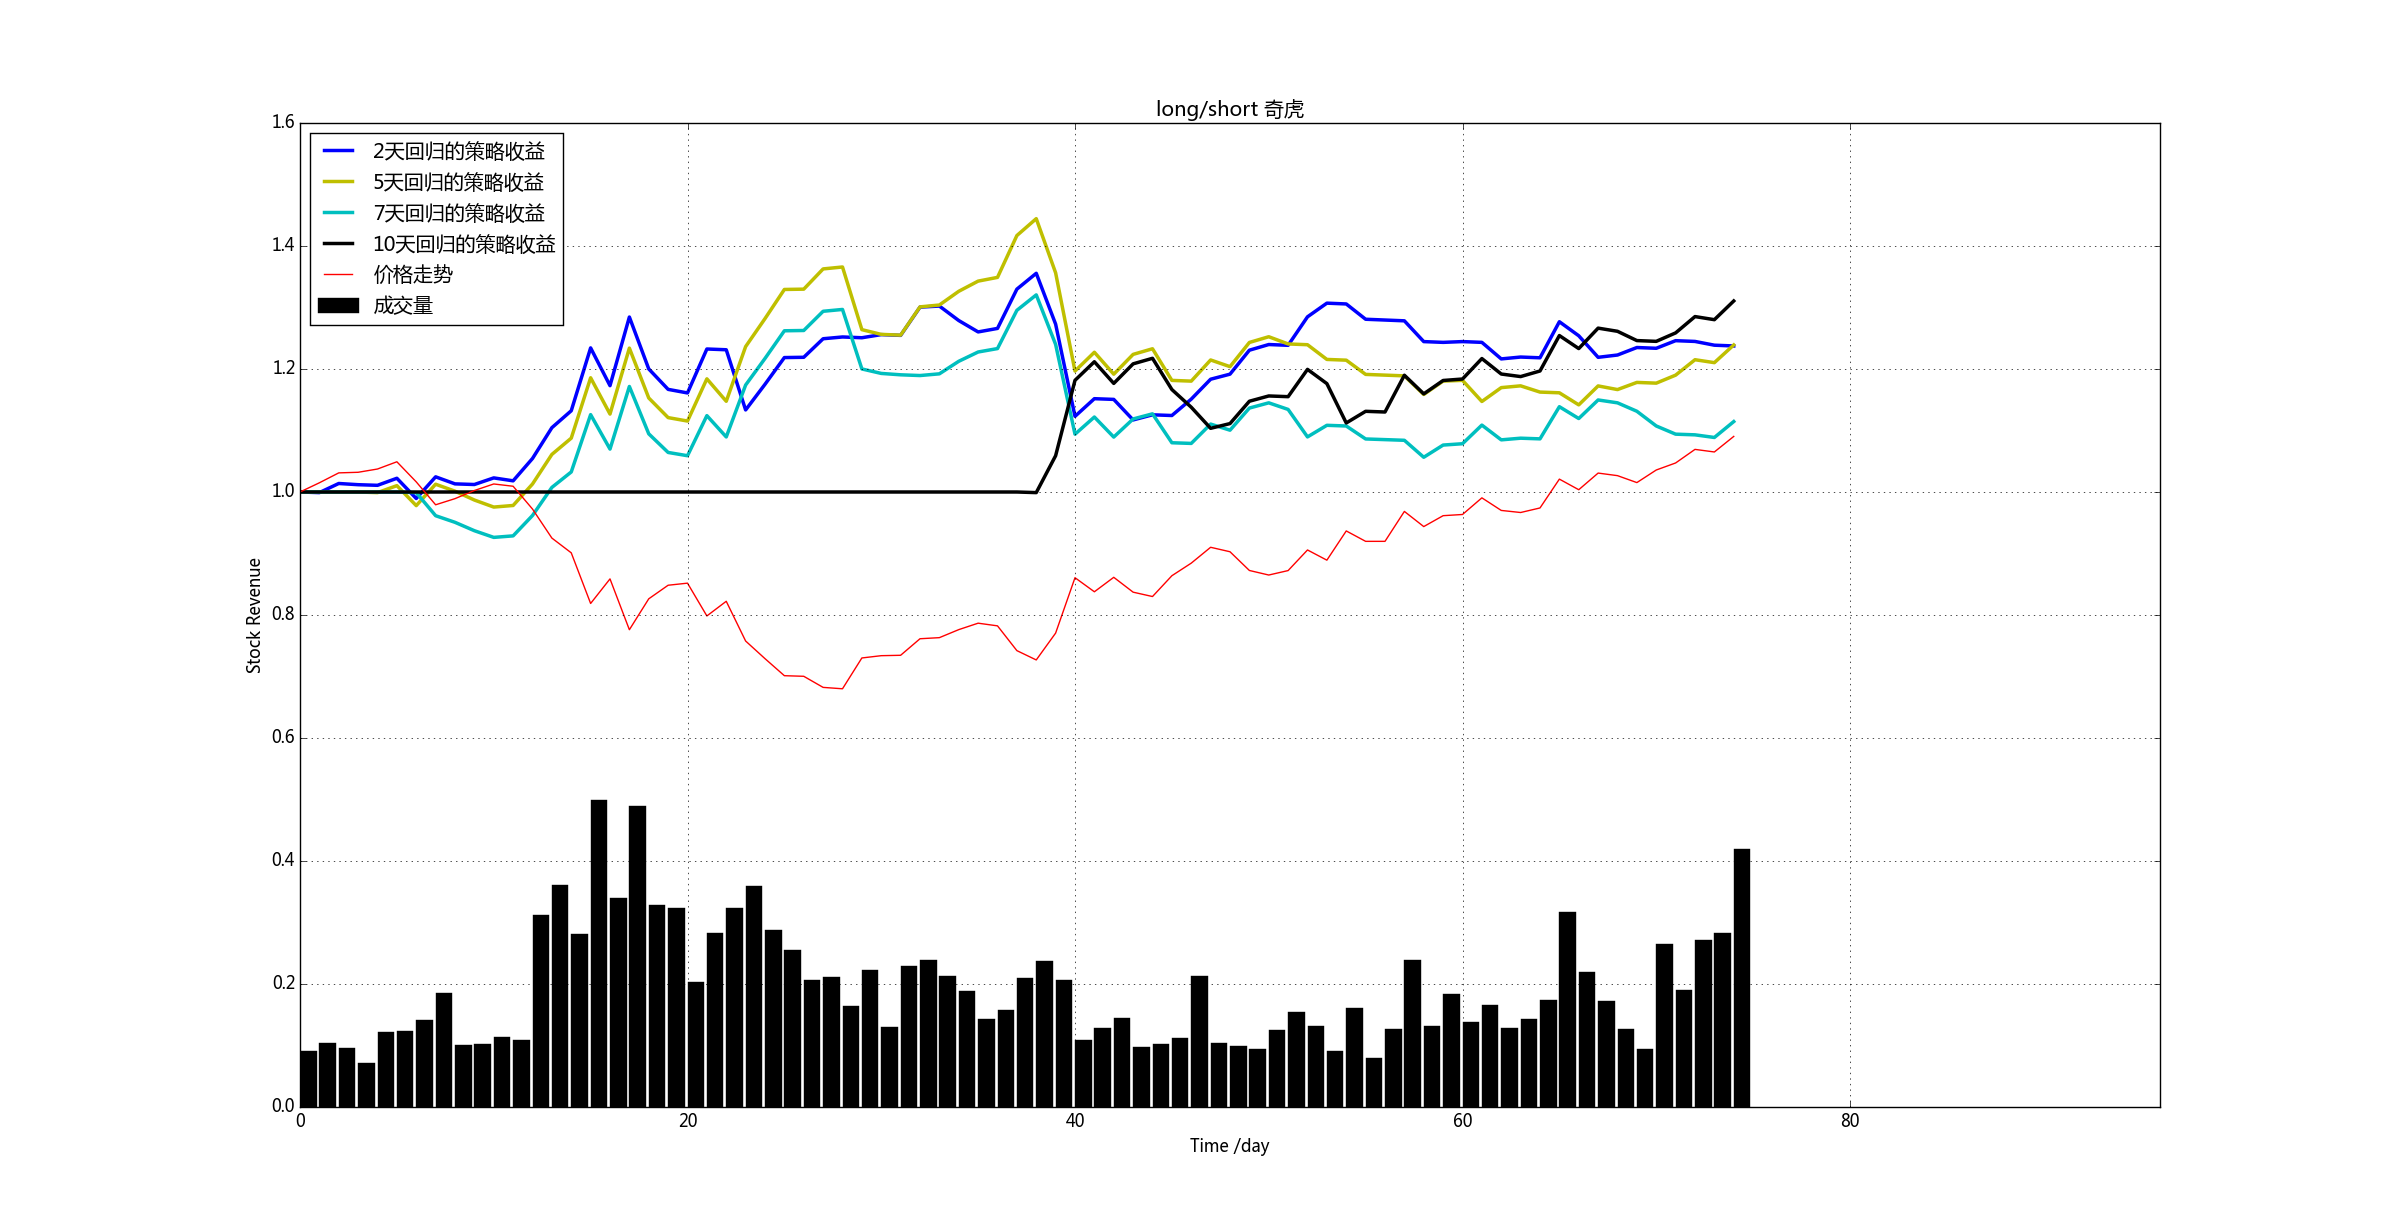
\includegraphics[width=1.0\textwidth]{img_r_1/short/qihu.png}
	\caption{奇虎 long/short}
\end{figure}

\item 奇虎 long/hold

\begin{figure}[H]
	\centering
	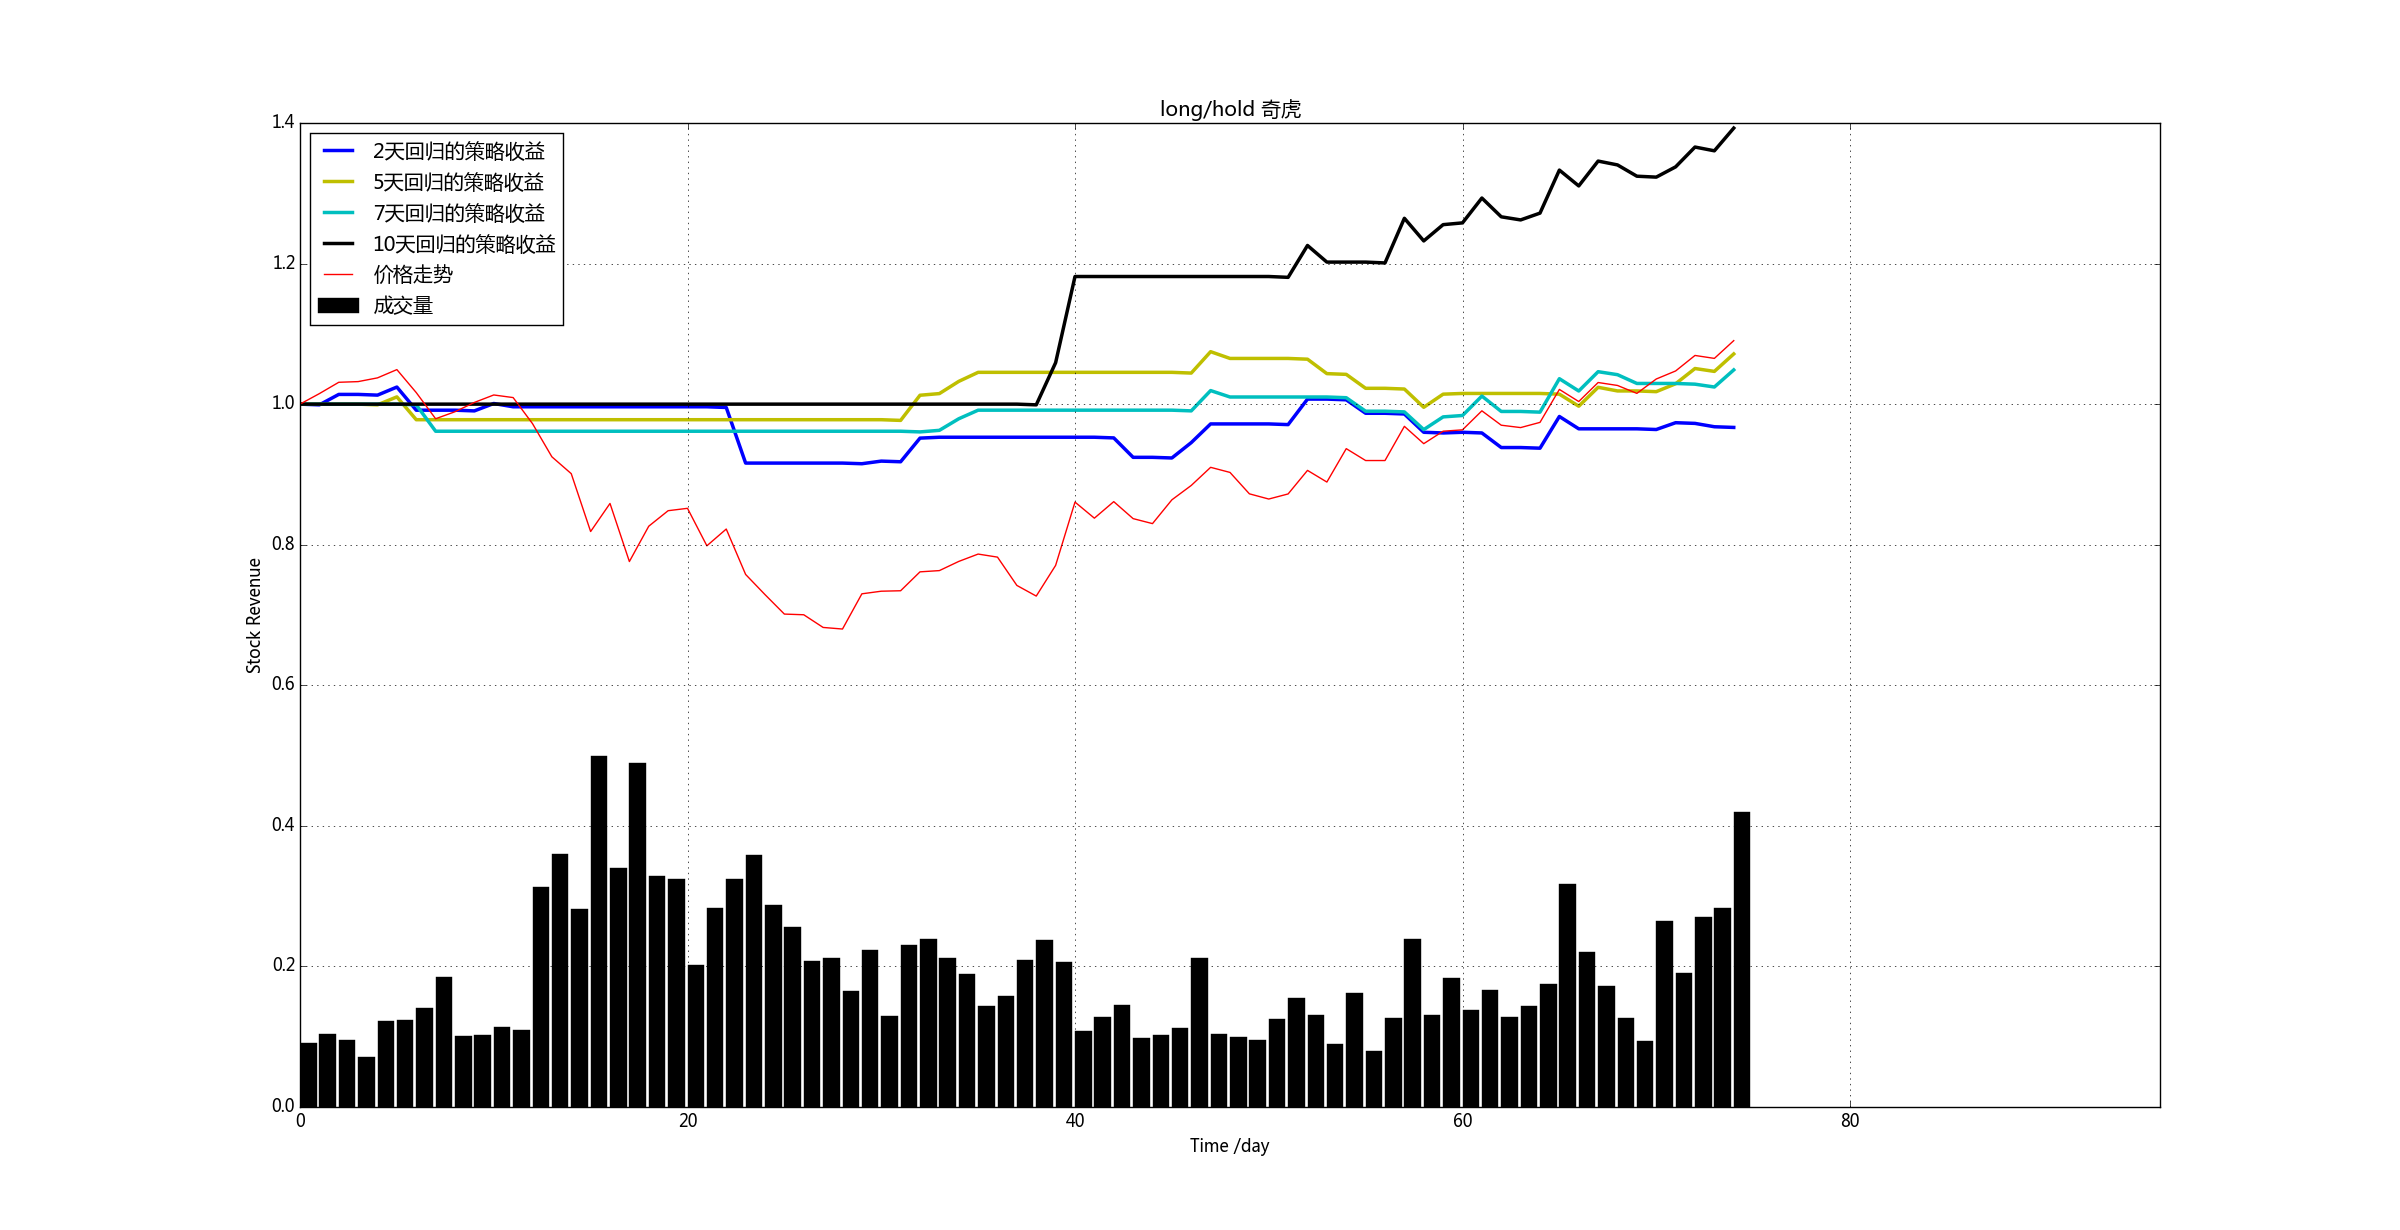
\includegraphics[width=1.0\textwidth]{img_r_1/hold/qihu.png}
	\caption{奇虎 long/hold}
\end{figure}

\end{enumerate}


\subsubsection{价格和成交量2日MA}

\begin{enumerate}[1.]
\item 惠理 long/short


\begin{figure}[H]
	\centering
	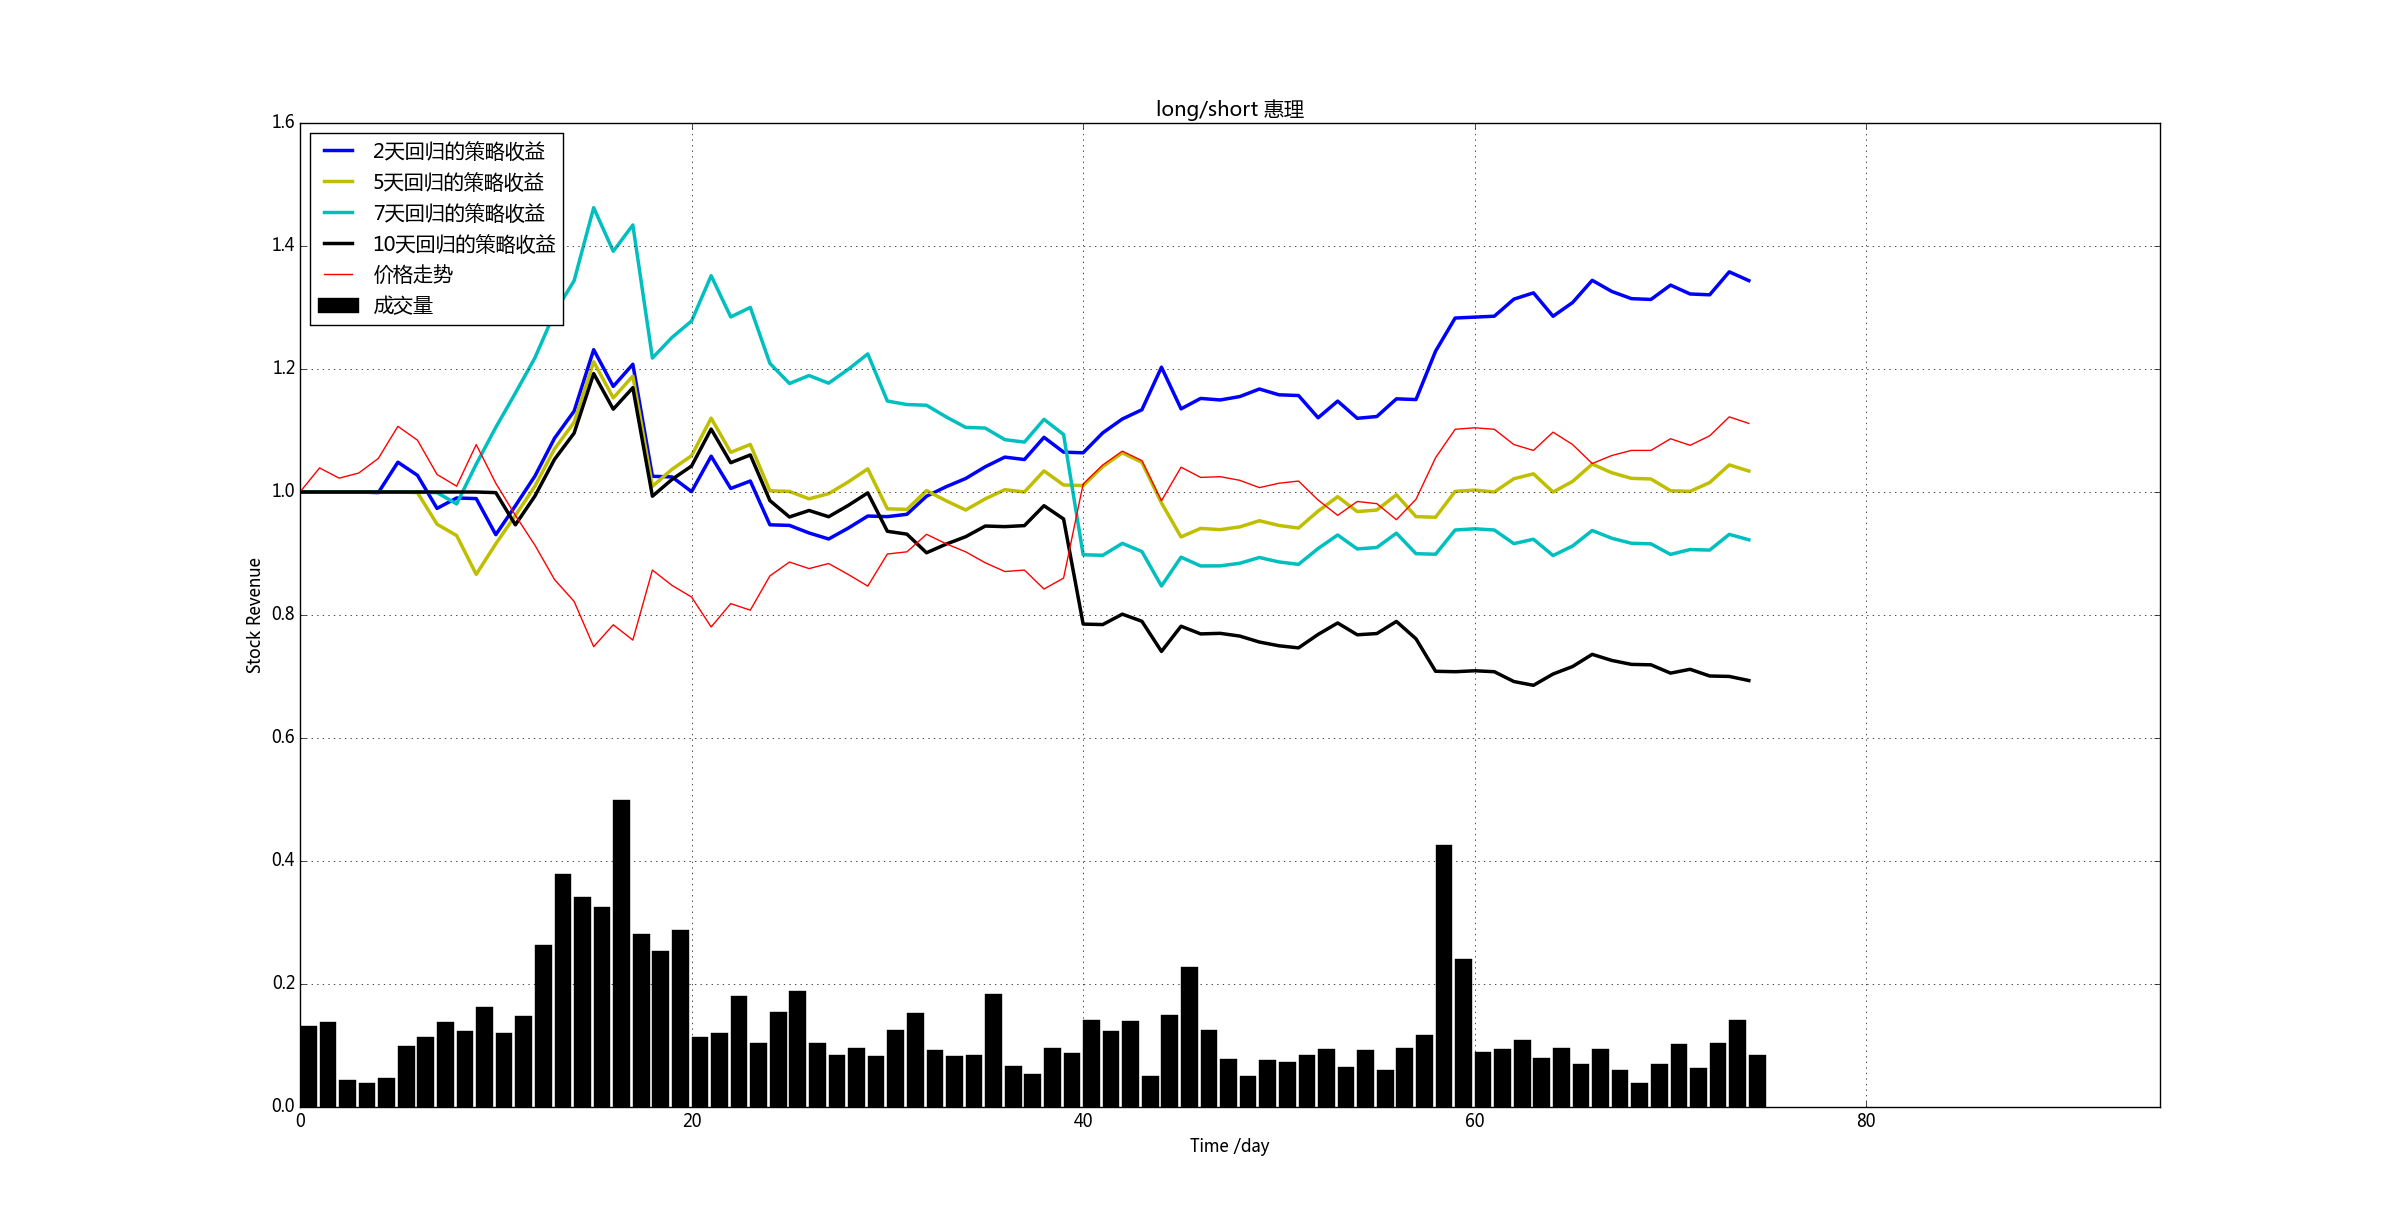
\includegraphics[width=1.0\textwidth]{img_r_2/short/hl.png}
	\caption{惠理 long/short}
\end{figure}

\item 惠理 long/hold

\begin{figure}[H]
	\centering
	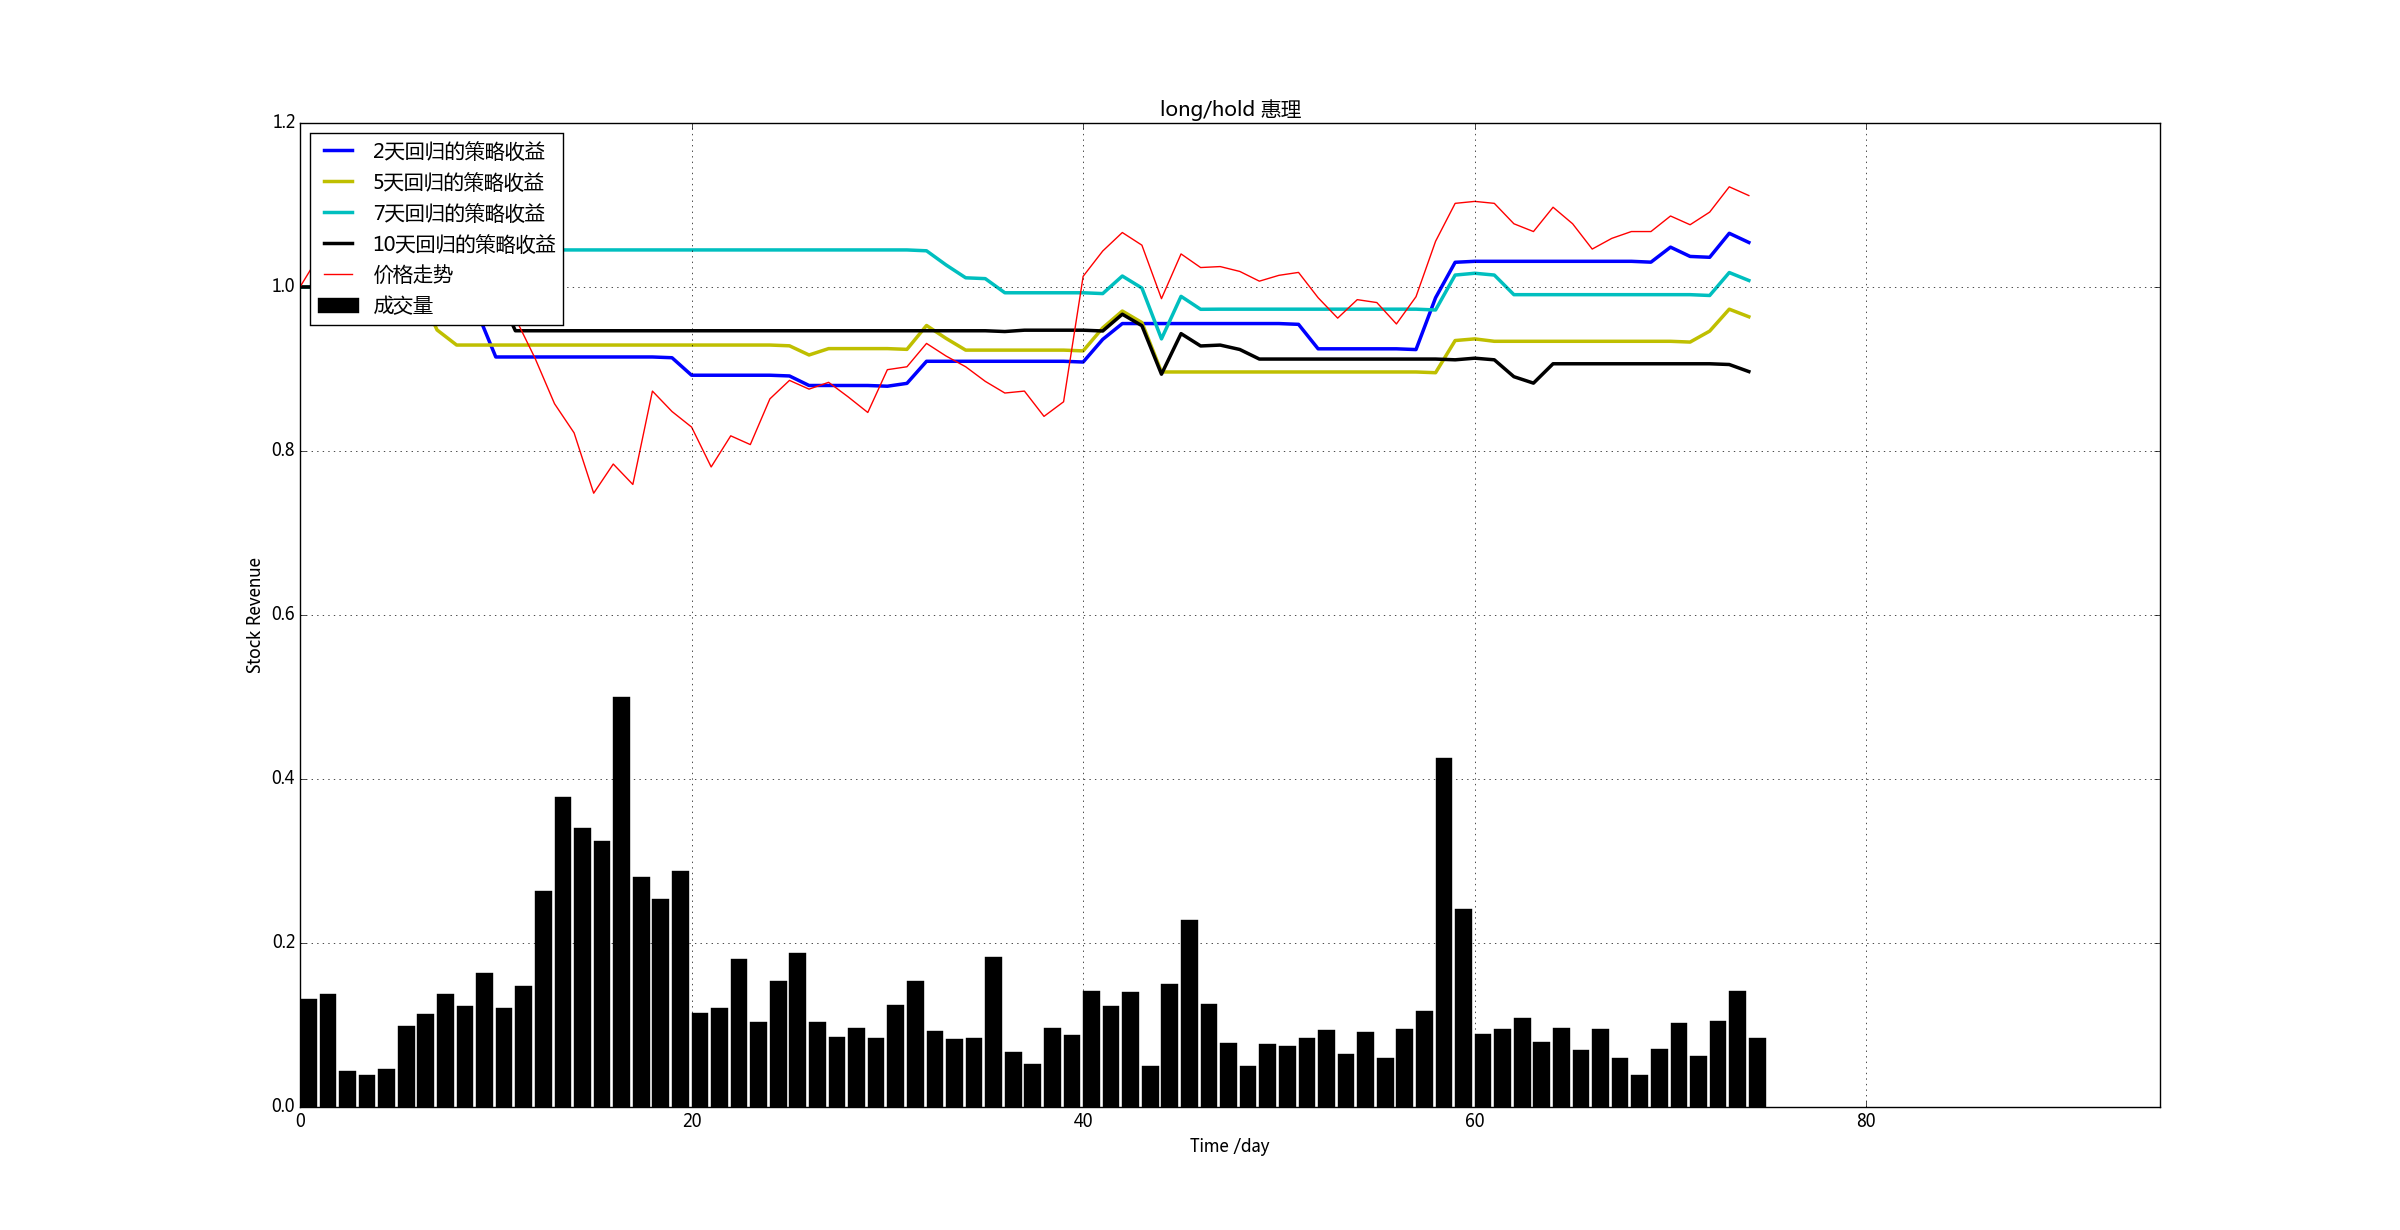
\includegraphics[width=1.0\textwidth]{img_r_2/hold/hl.png}
	\caption{惠理 long/hold }
\end{figure}

\item 奇虎 long/short


\begin{figure}[H]
	\centering
	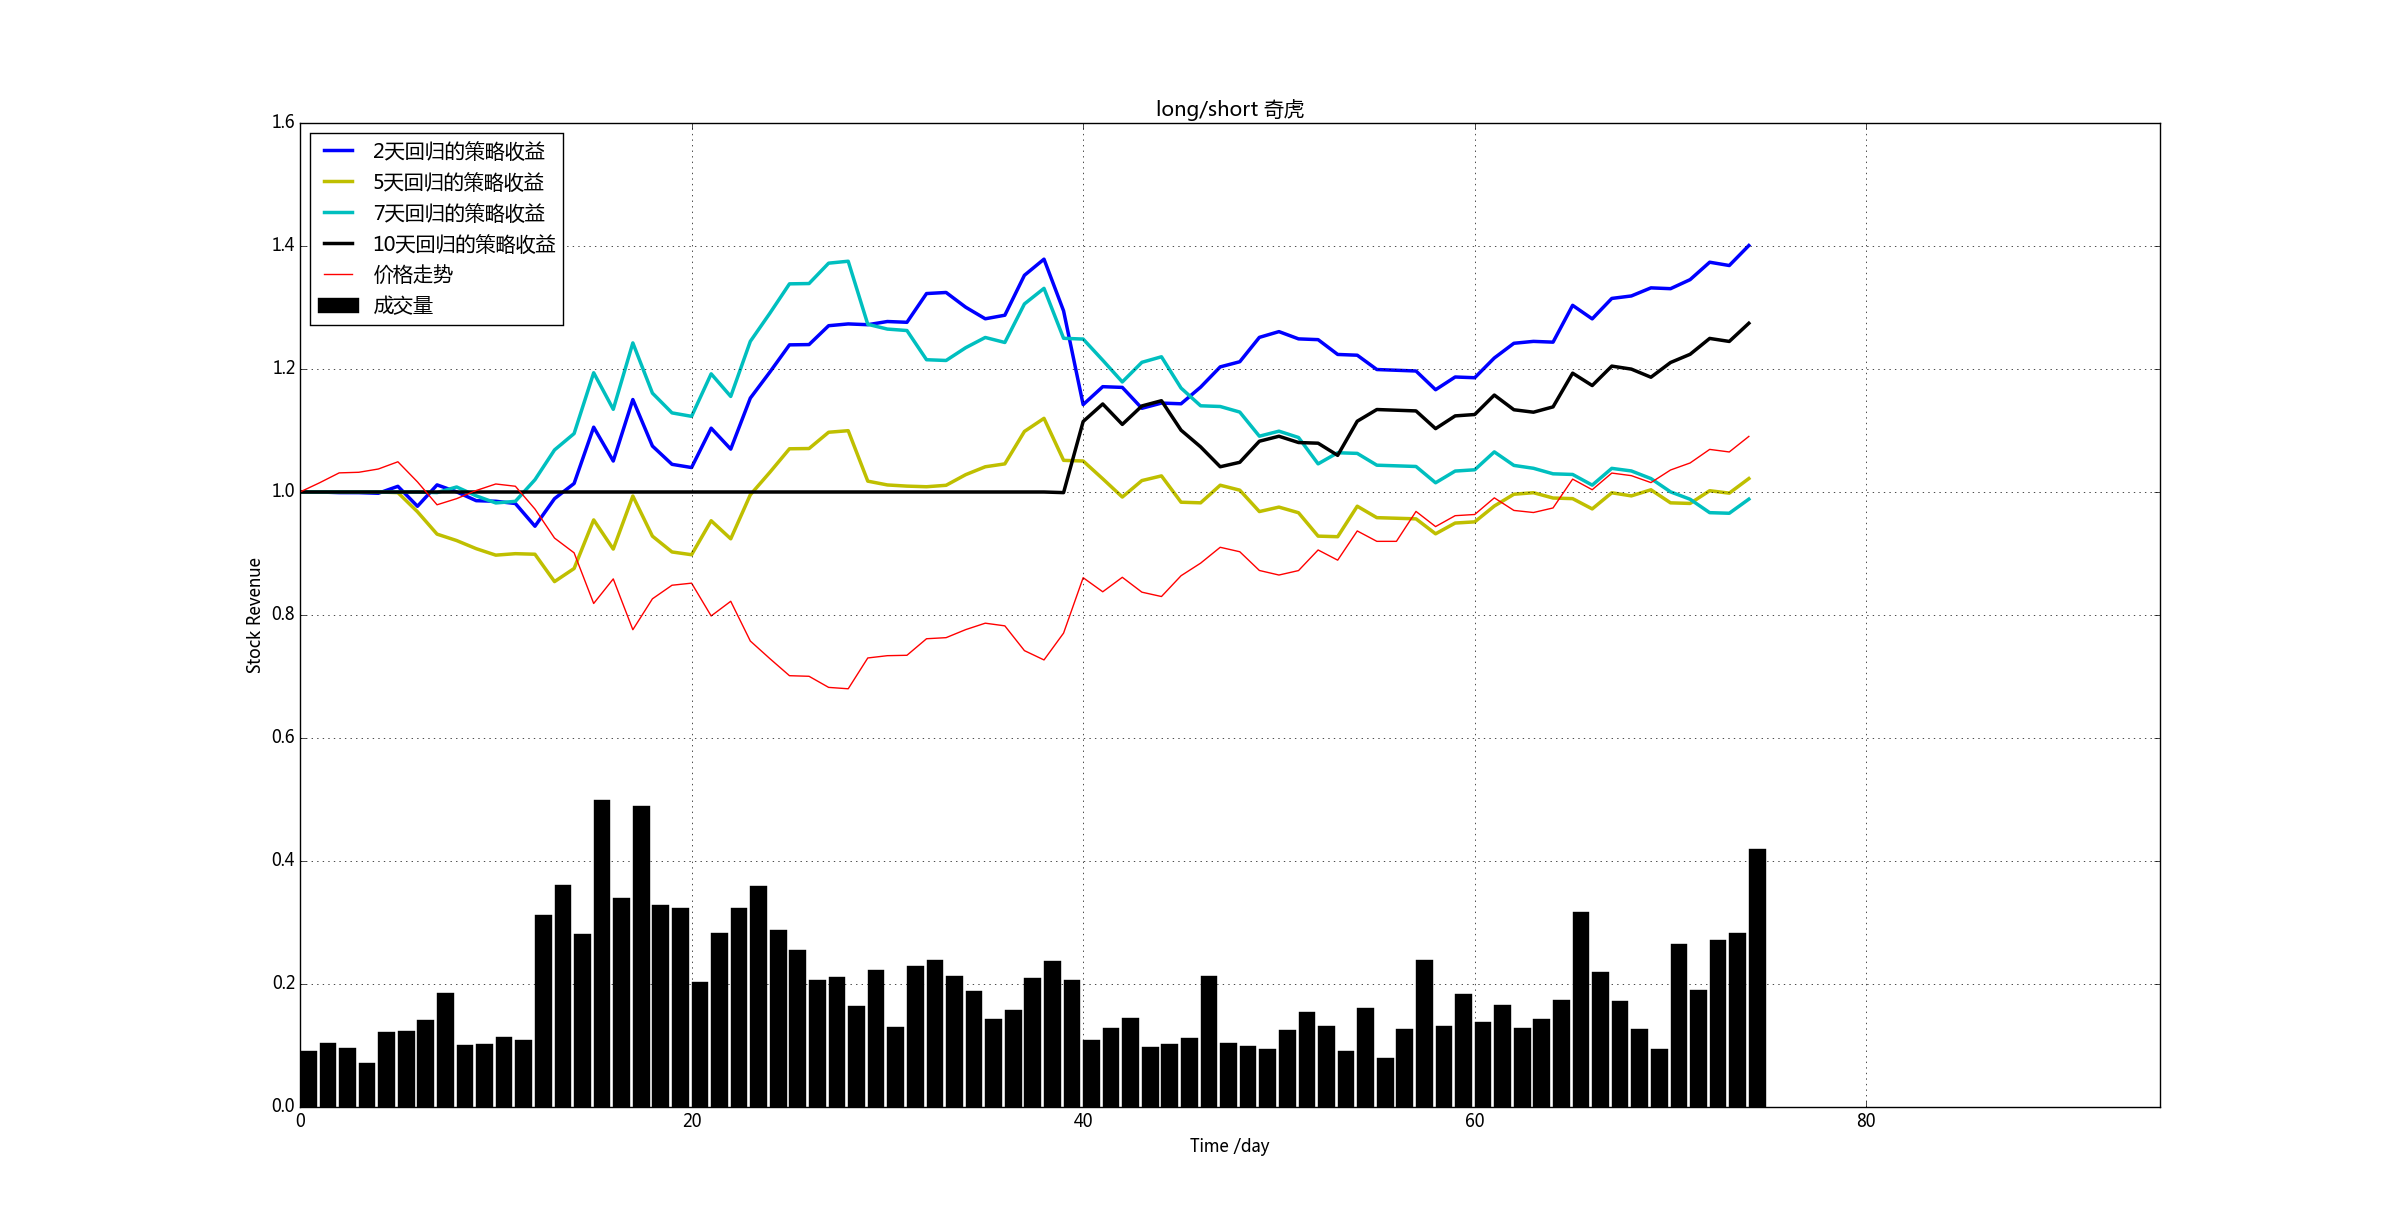
\includegraphics[width=1.0\textwidth]{img_r_2/short/qihu.png}
	\caption{奇虎 long/short}
\end{figure}

\item 奇虎 long/hold

\begin{figure}[H]
	\centering
	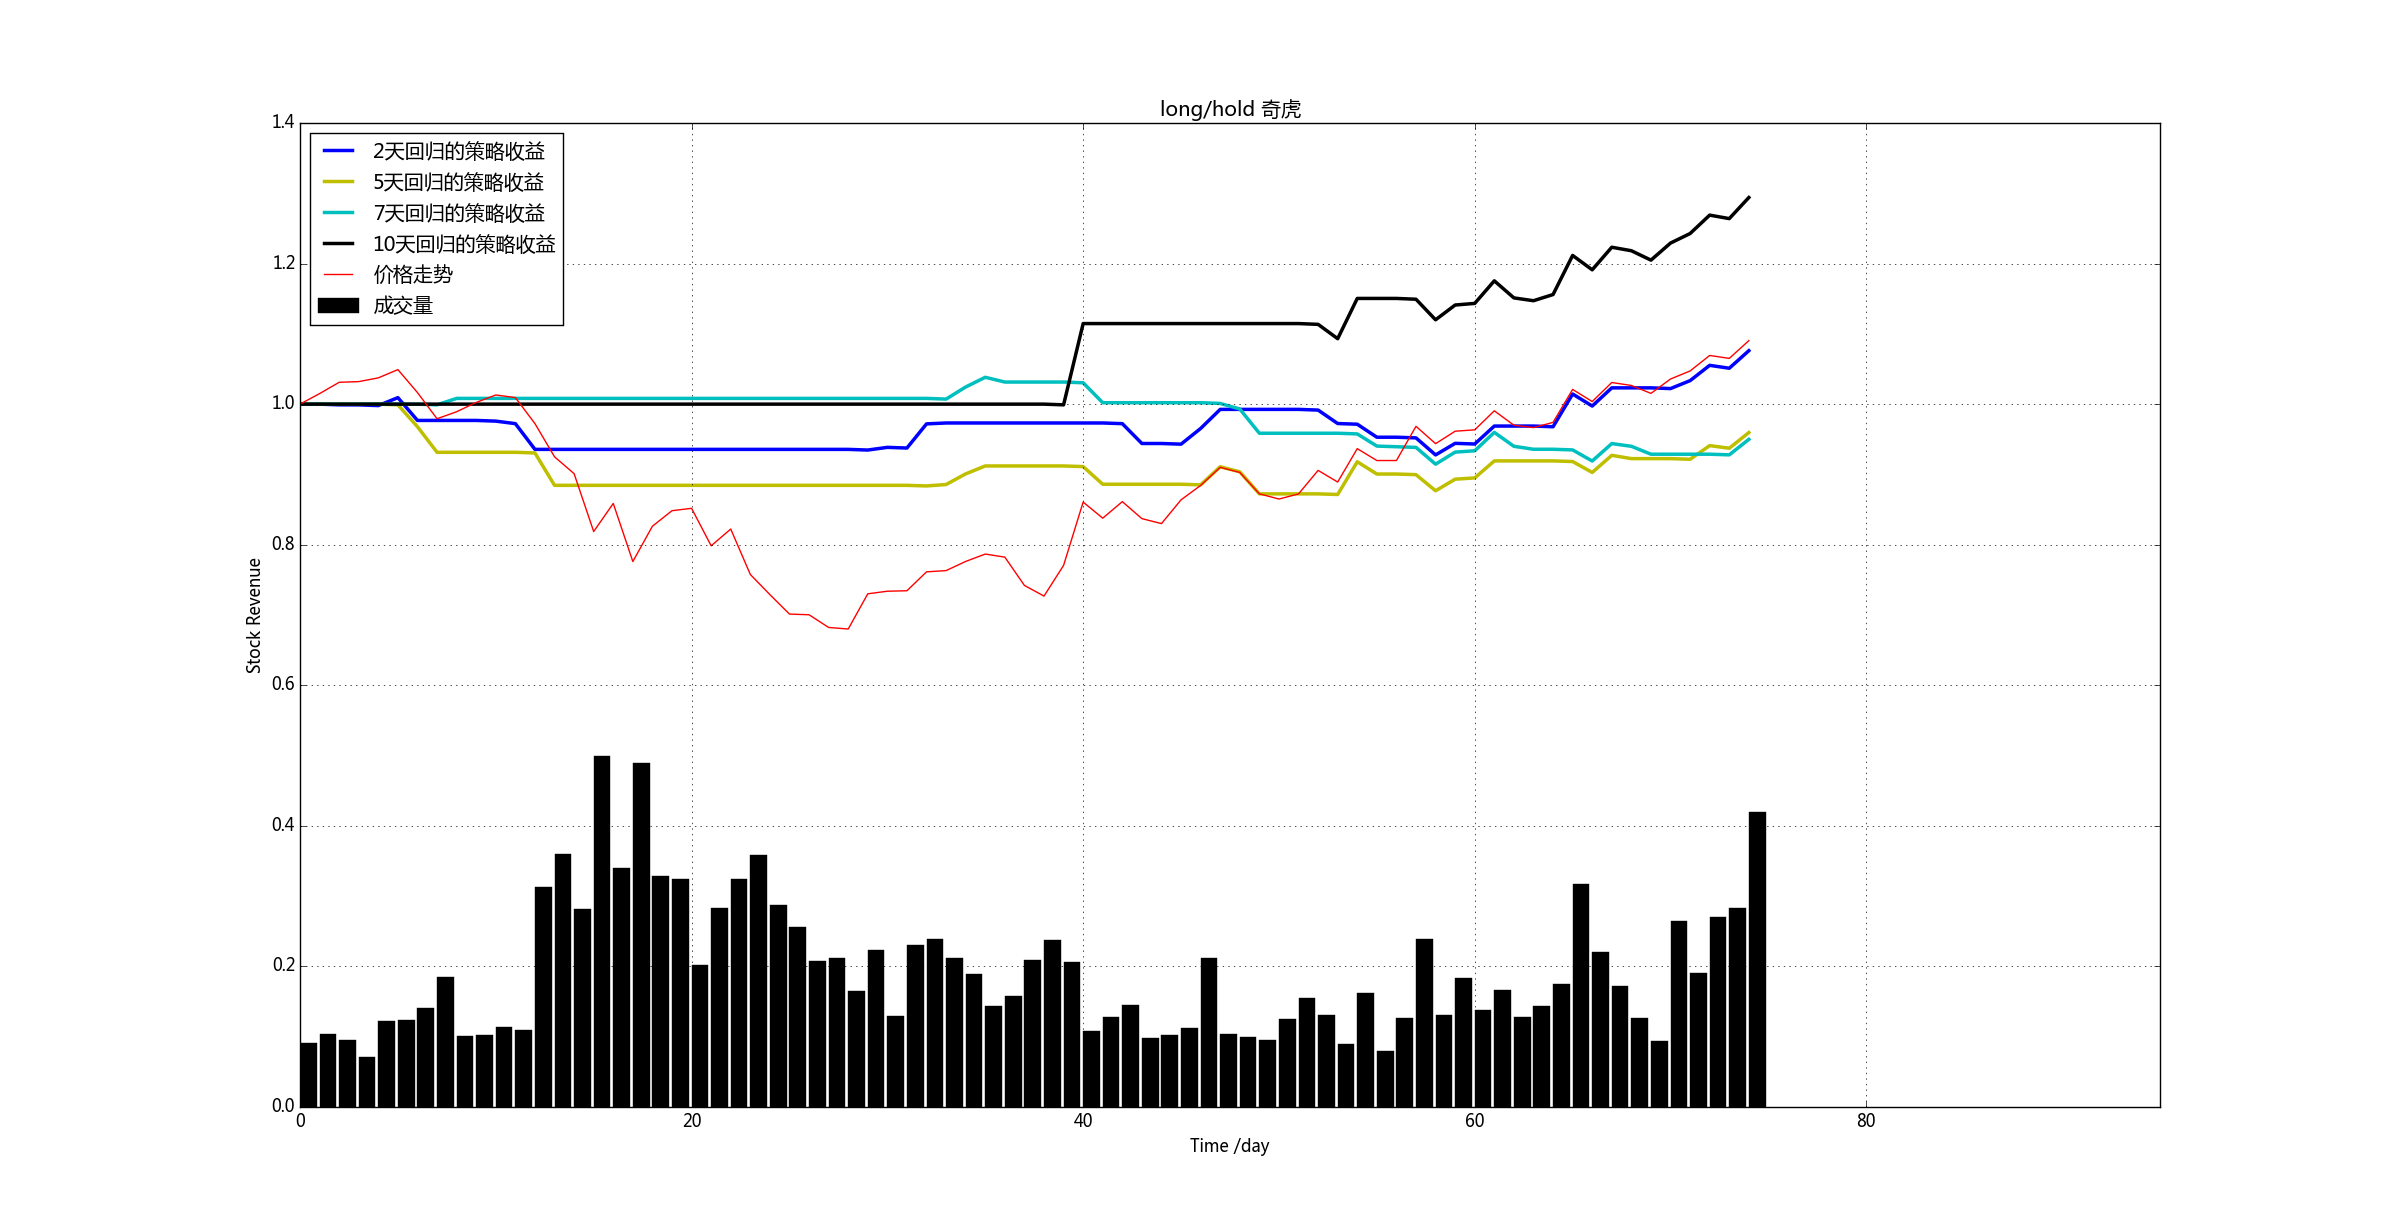
\includegraphics[width=1.0\textwidth]{img_r_2/hold/qihu.png}
	\caption{奇虎 long/hold}
\end{figure}

\end{enumerate}

\subsubsection{价格和成交量5日MA}

\begin{enumerate}[1.]
\item 惠理 long/short


\begin{figure}[H]
	\centering
	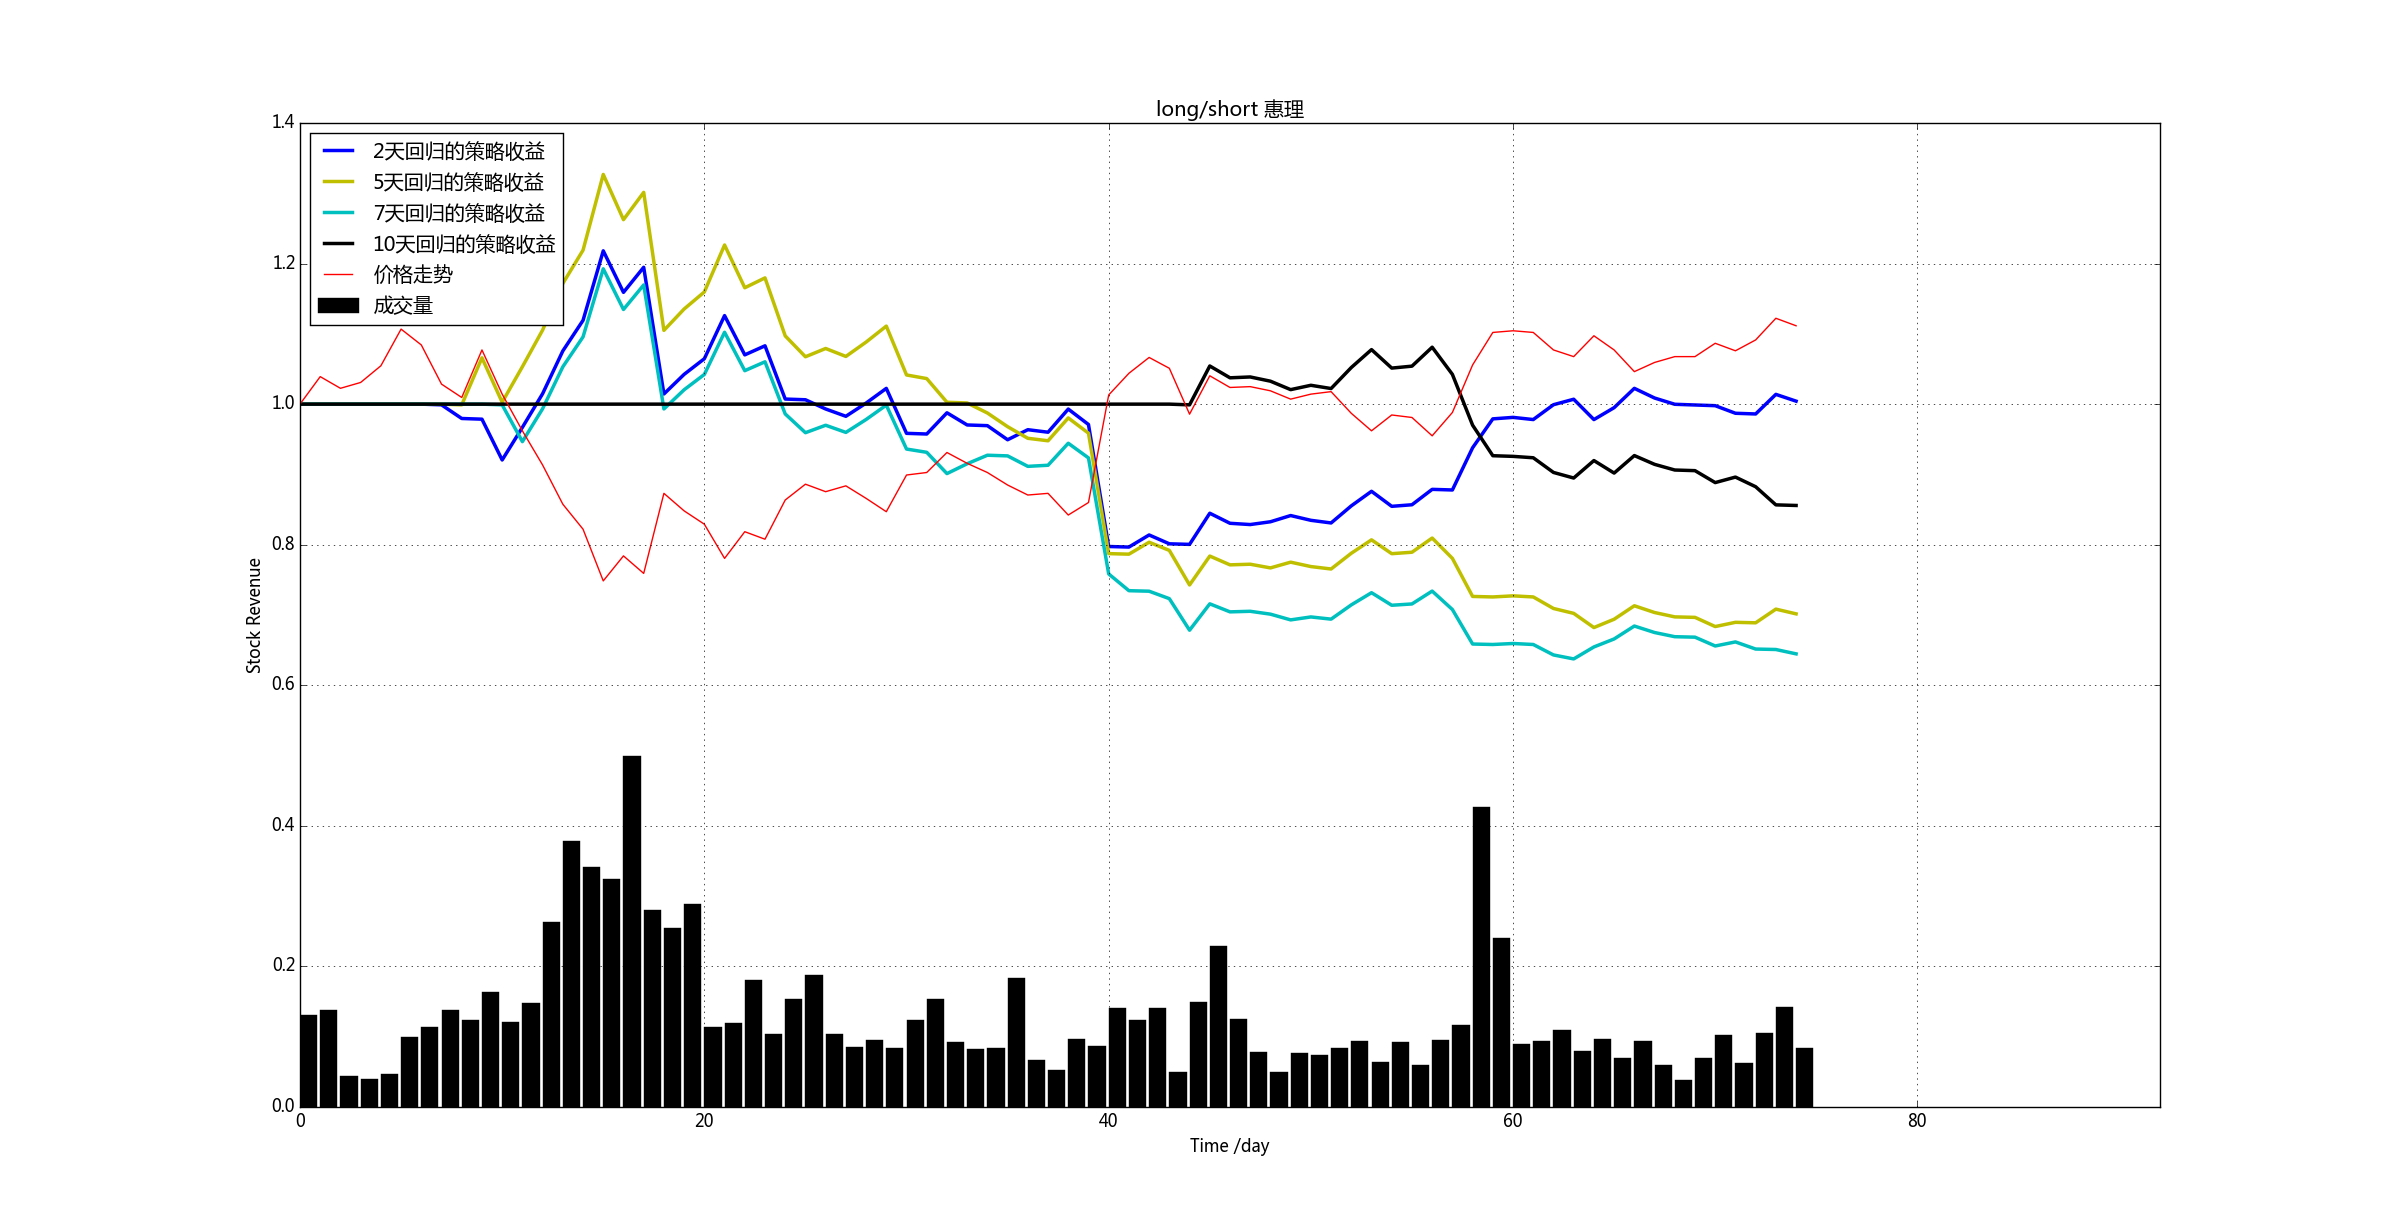
\includegraphics[width=1.0\textwidth]{img_r_5/short/hl.png}
	\caption{惠理 long/short }
\end{figure}

\item 惠理 long/hold

\begin{figure}[H]
	\centering
	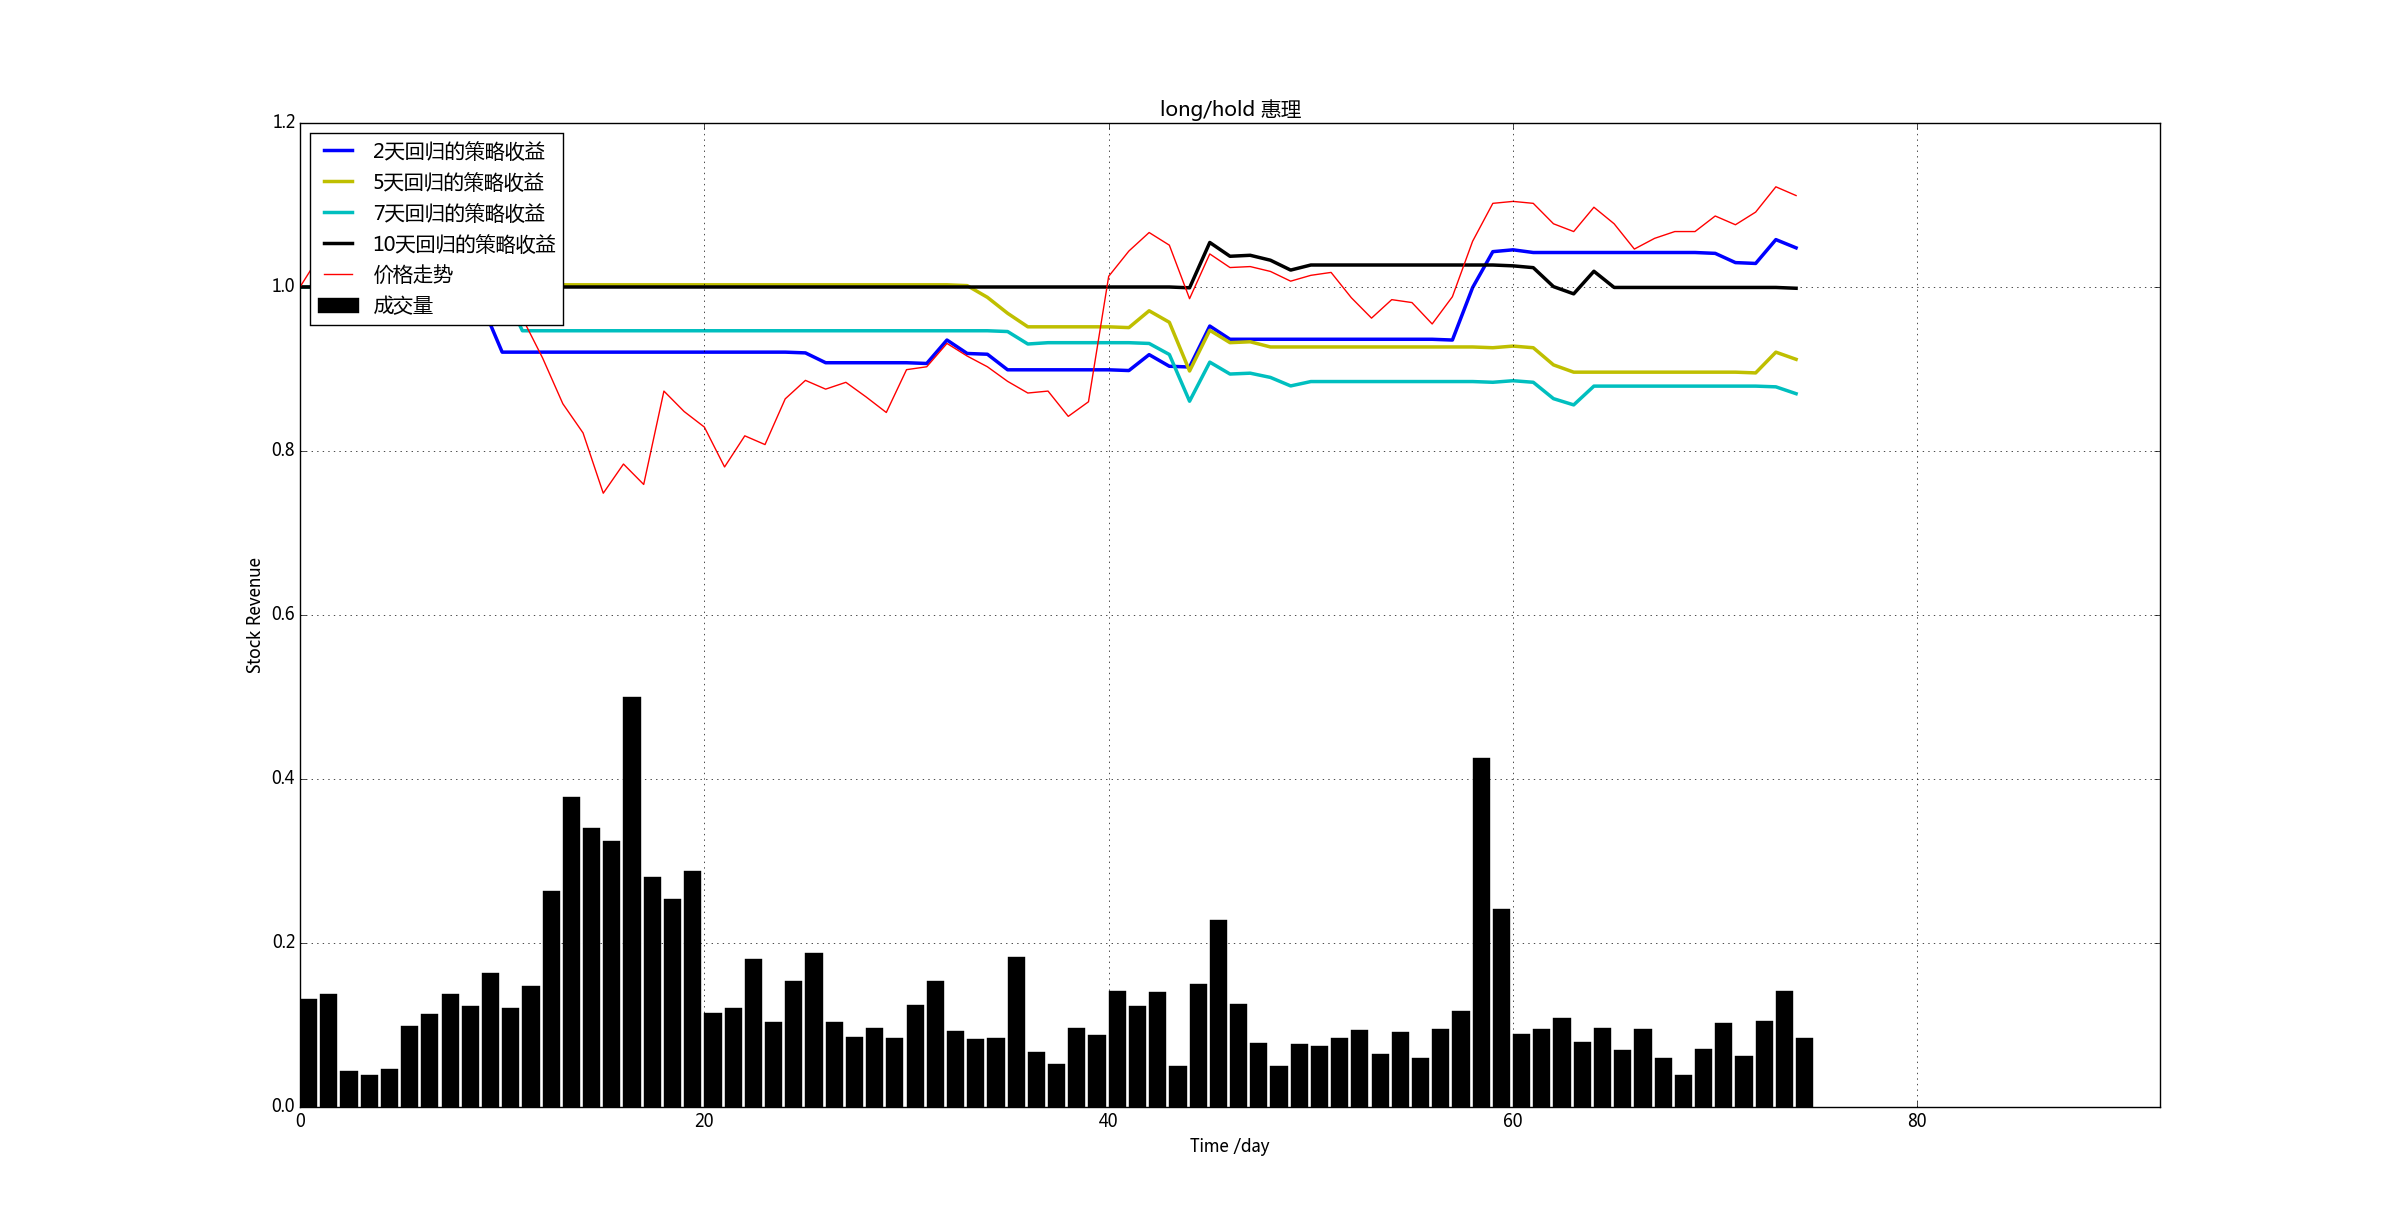
\includegraphics[width=1.0\textwidth]{img_r_5/hold/hl.png}
	\caption{惠理 long/hold}
\end{figure}

\item 奇虎 long/short


\begin{figure}[H]
	\centering
	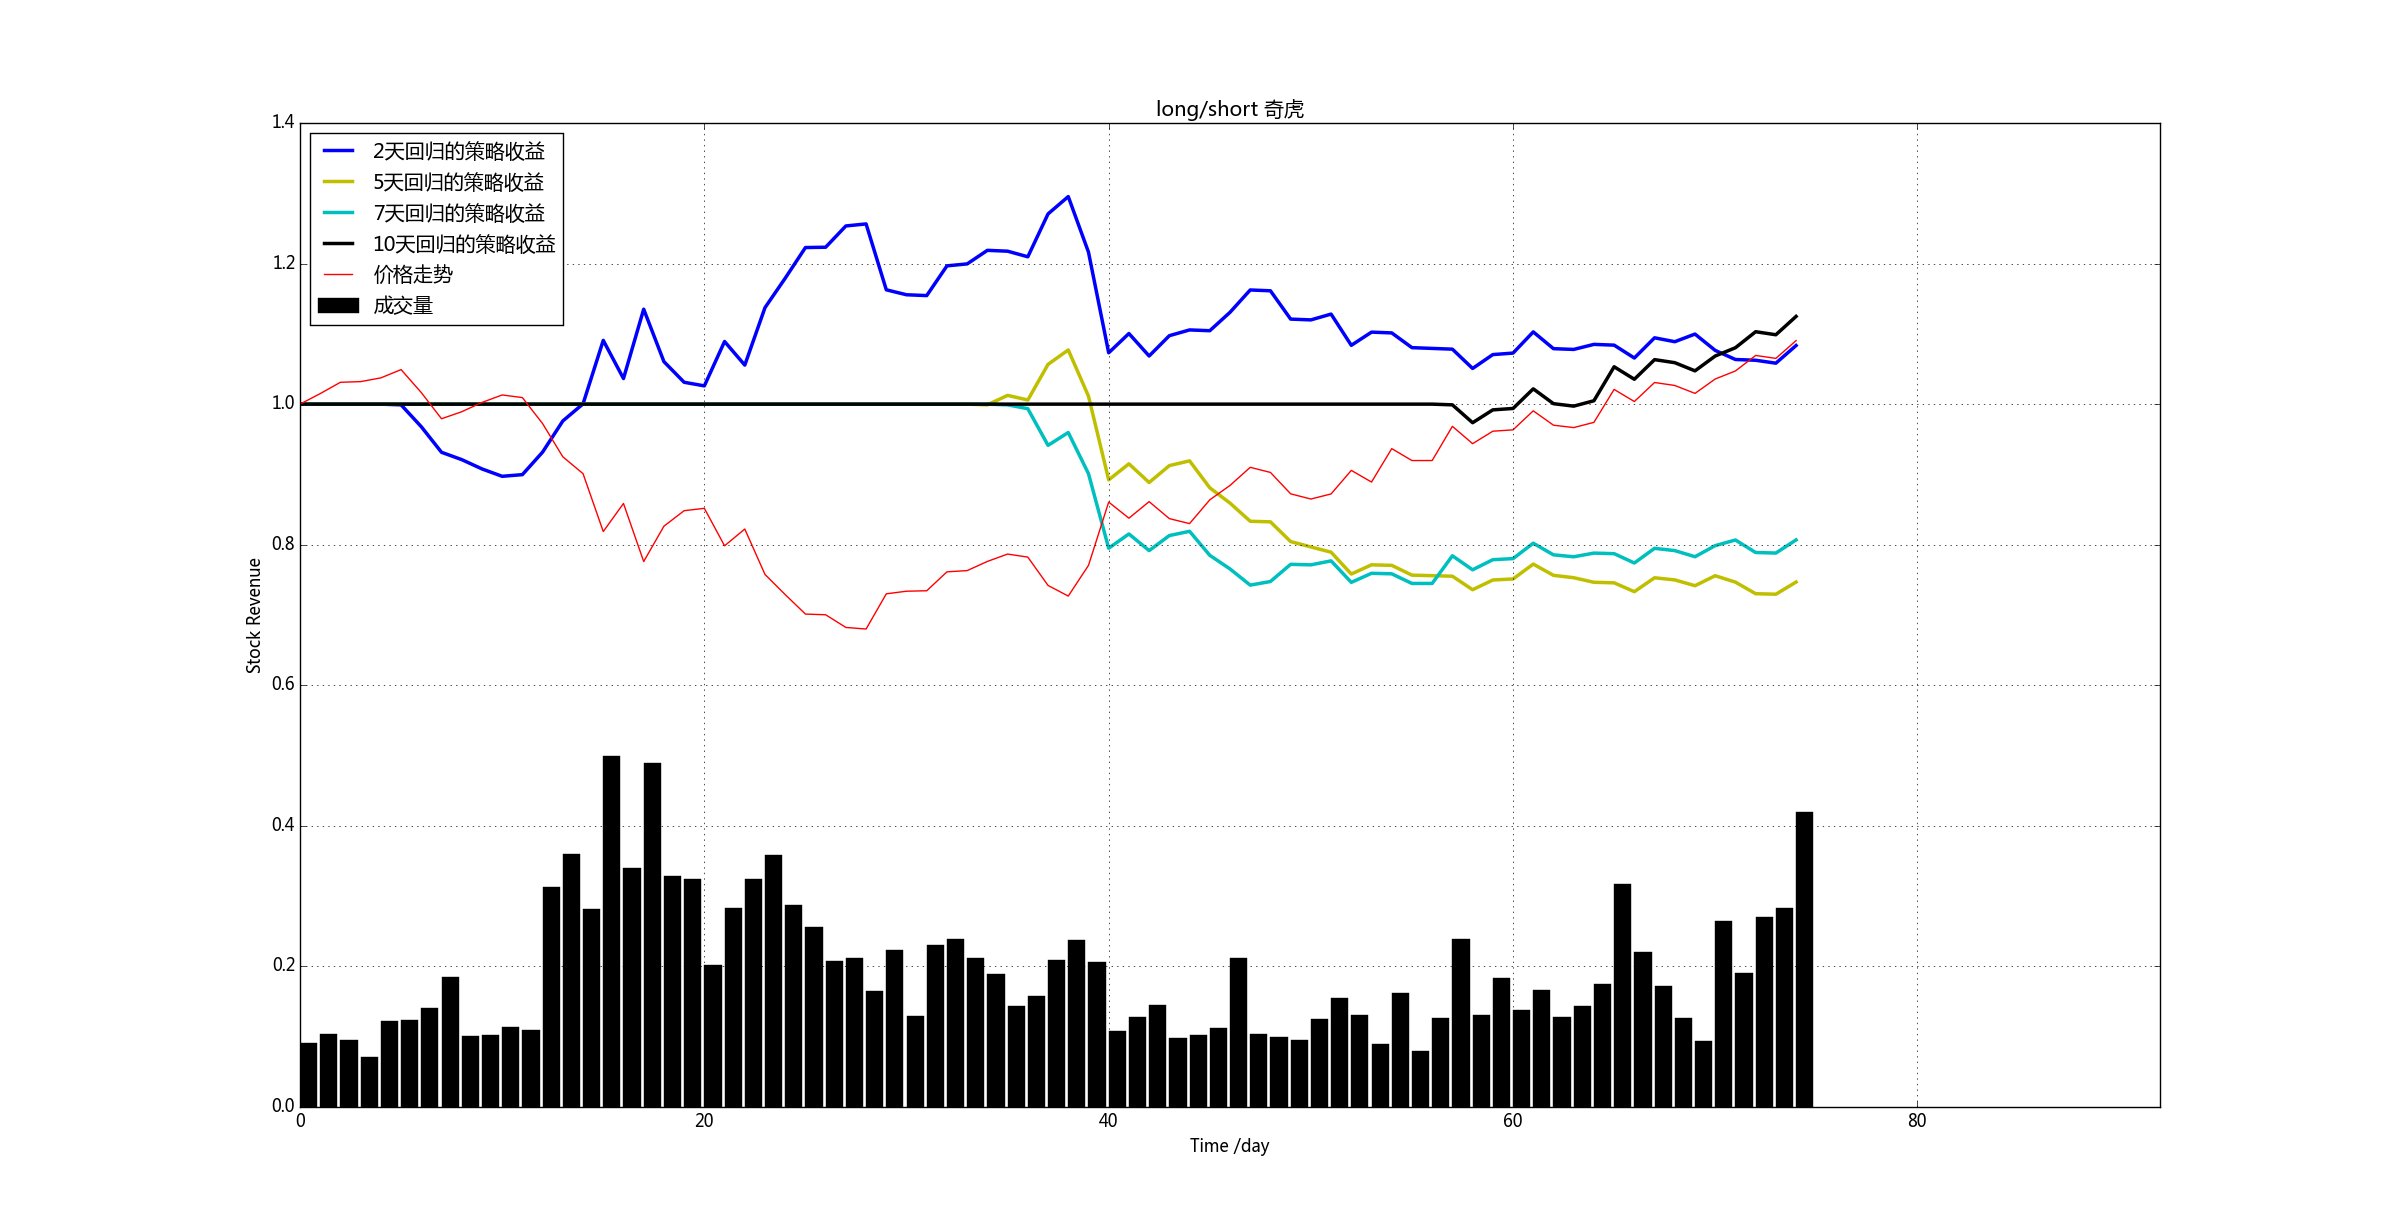
\includegraphics[width=1.0\textwidth]{img_r_5/short/qihu.png}
	\caption{奇虎 long/short}
\end{figure}

\item 奇虎 long/hold

\begin{figure}[H]
	\centering
	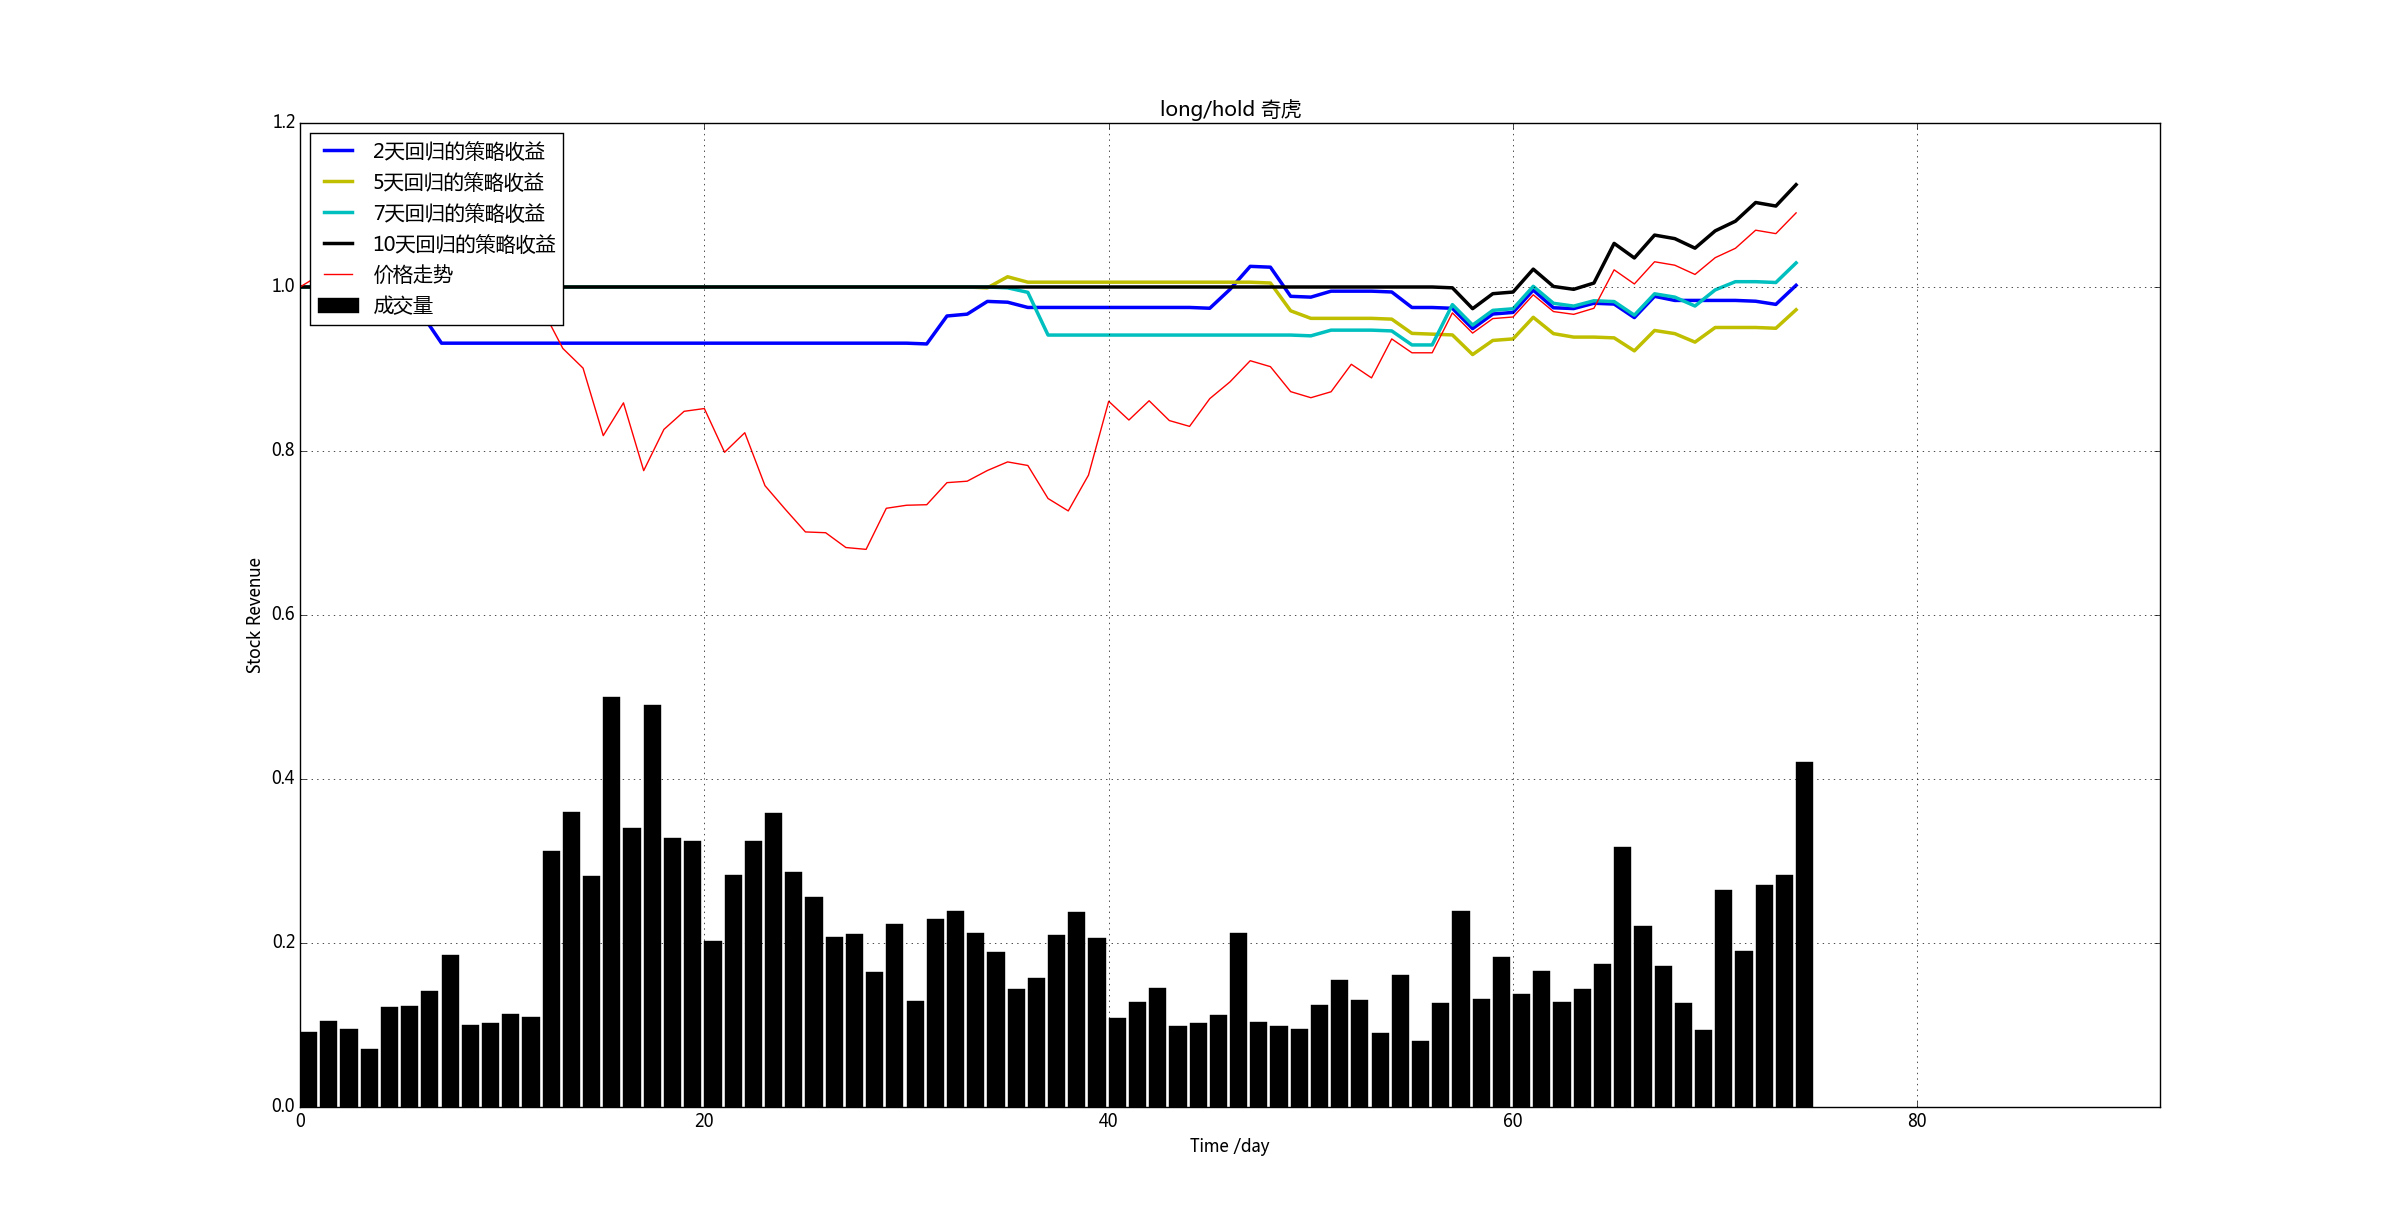
\includegraphics[width=1.0\textwidth]{img_r_5/hold/qihu.png}
	\caption{奇虎 long/hold}
\end{figure}

\end{enumerate}





\subsection{回测结果分析}

\subsubsection{4天动量模型}

\begin{enumerate}
\item 该策略在惠理上的回测结果较糟糕;
\item 该策略在奇虎大跌时效果较好,上涨阶段效果很差。
\item 该策略适合缓慢单边上涨的情况,如果中途有较大回调,则会影响效果,甚至做错方向。(参见奇虎9月底的回调及策略结果)
\item 该策略在大跌时,往往效果不错。(参加惠理和奇虎在8月下旬的下跌及策略结果)

\end{enumerate}
\subsubsection{量价模型}
\begin{enumerate}
\item 2天回归的策略在惠理上效果较好;10天回归的策略在奇虎上效果较好
\item 该策略的回归周期较长的时候(比如10天),能够抓住单边上涨(奇虎9月之后的上涨)
\item 对惠理没有找到很好的解释

\end{enumerate}




\end{document}